% !TEX encoding = UTF-8
% !TEX TS-program = pdflatex
% !TEX root = ../tesi.tex

%**************************************************************
\chapter{Sviluppo}
\label{cap:sviluppo}
Il capitolo descrive le attività svolte e le principali difficoltà incontrate durate lo sviluppo delle applicazioni. Per prima verrà trattata l'applicazione cliente, in seguito l'applicazione coach e saranno disponibili gli screenshot dei risultati finali ottenuti.\\
La codifica è avvenuta per moduli: prima di passare al modulo successivo il risultato è stato visionato dall’azienda e dal tutor.\\
Saranno riportati solamente gli esempi di codice ritenuti più significativi.
%**************************************************************

\section{integrazione asa in ar flut plug}
La prima cosa su cui si è lavorato è stato il sistema di login e di recupero delle informazioni del cliente.\\
Una volta ricevuto dal mio tutor il \textit{provider} che si occupa del login tramite \textit{Auth0} sono stati sviluppati diversi widget per gestire il routing dell'applicazione in base al login avvenuto con successo o meno.\\
Inoltre è stato definito un modello per memorizzare i dati dell'utente ricevuto tramite chiamata API.
%*************************************************************************
\subsection{ar flutter plugin mobilesyn}
Per gestire il routing iniziale dell'applicazione si è deciso di sviluppare multipli widget \textit{statefull} in ascolto sullo stato di diverse richieste API, così facendo, al cambiamento di stato della richiesta API il widget viene ricostruito e indirizza l'applicazione ad un widget successivo in ascolto su di un'altra chiamata API. Questa opzione è stata scelta in quanto all'avvio dell'applicazione vengono eseguite diverse chiamate API e in questo modo è possibile osservare i campi \textit{Loading} ed \textit{Error}, come spiegato a sezione 4.3.3, in modo da avere un controllo sul flusso.\\
Di seguito elenco la lista di widget con i diversi instradamenti.\\
\begin{itemize}
    \item \textbf{MyApp}: prova l'autenticazione e finché il provider di autenticazione resta nello stato di \textit{Loading} mostra una \textit{SplashScreen}, successivamente indirizza verso il widget \textbf{CheckLogin};
    \item \textbf{CheckLogin}: controlla se l'accesso è avvenuto con successo o meno. Se si, in base al tipo di applicazione (client o coach) indirizza al widget \textbf{LoadUser} o \textit{LoadCoach}, se l'accesso è fallito indirizza alla \textbf{LoginScreen};
    \item \textbf{LoginScreen}: widget per riprovare l'accesso inserendo username e password;
    \item LoadUser: richiede al backend le informazioni dell'utente che ha effettuato l'accesso e mostra una schermata di caricamento mentre la chiamata è in stato di \textit{Loading}, successivamente indirizza al widget \textbf{CheckBoolUser};
    \item \textbf{CheckBoolUser}: controlla se è il primo accesso dell'utente o meno, se lo è indirizza ad una schermata con l'introduzione all'applicazione, altrimenti riporta alla schermata di \textit{Homepage}.
    \item \textbf{LoadCoach}: richiede al backend le informazioni del coach che ha effettuato l'accesso e mostra una schermata di caricamento mentre la chiamata è in stato di \textit{Loading}, successivamente indirizza al widget \textbf{CheckBoolCoach};
    \item \textbf{CheckBoolUser}: controlla se ci sono stati errori nel recupero delle informazioni, se ci sono stati restituisce un widget di errore, altrimenti riporta alla schermata di \textit{Homepage}.
\end{itemize}

\begin{lstlisting}[language=dart, firstnumber=1, caption={Widget CheckLogin}]
class CheckLogin extends HookWidget {
  @override
  Widget build(BuildContext context) {
    bool isLoggedIn = useProvider(authIsLoggedIn);
    bool error = useProvider(authError);
    String errorMsg = useProvider(authErrorMessage);
    if (error) return GenericErrorPage(errorMsg: errorMsg);
    if (!isLoggedIn) {
        return LoginScreen();
    } else {
      switch (envType) {
        case "client":
          return LoadUser();
        case "coach":
          return LoadCoach();
        default:
          return GenericErrorPage(errorMsg: "non sei ne coach ne client");
      }
    }
  }
}
\end{lstlisting}
%%%%%%%%%%%%%%%%%%%%%%%%%%%%%%%%%%%%%%%%%%%%%%%%%%%%%%%%
\begin{center}
\begin{figure}[H]
\subfloat[Splash Screen]{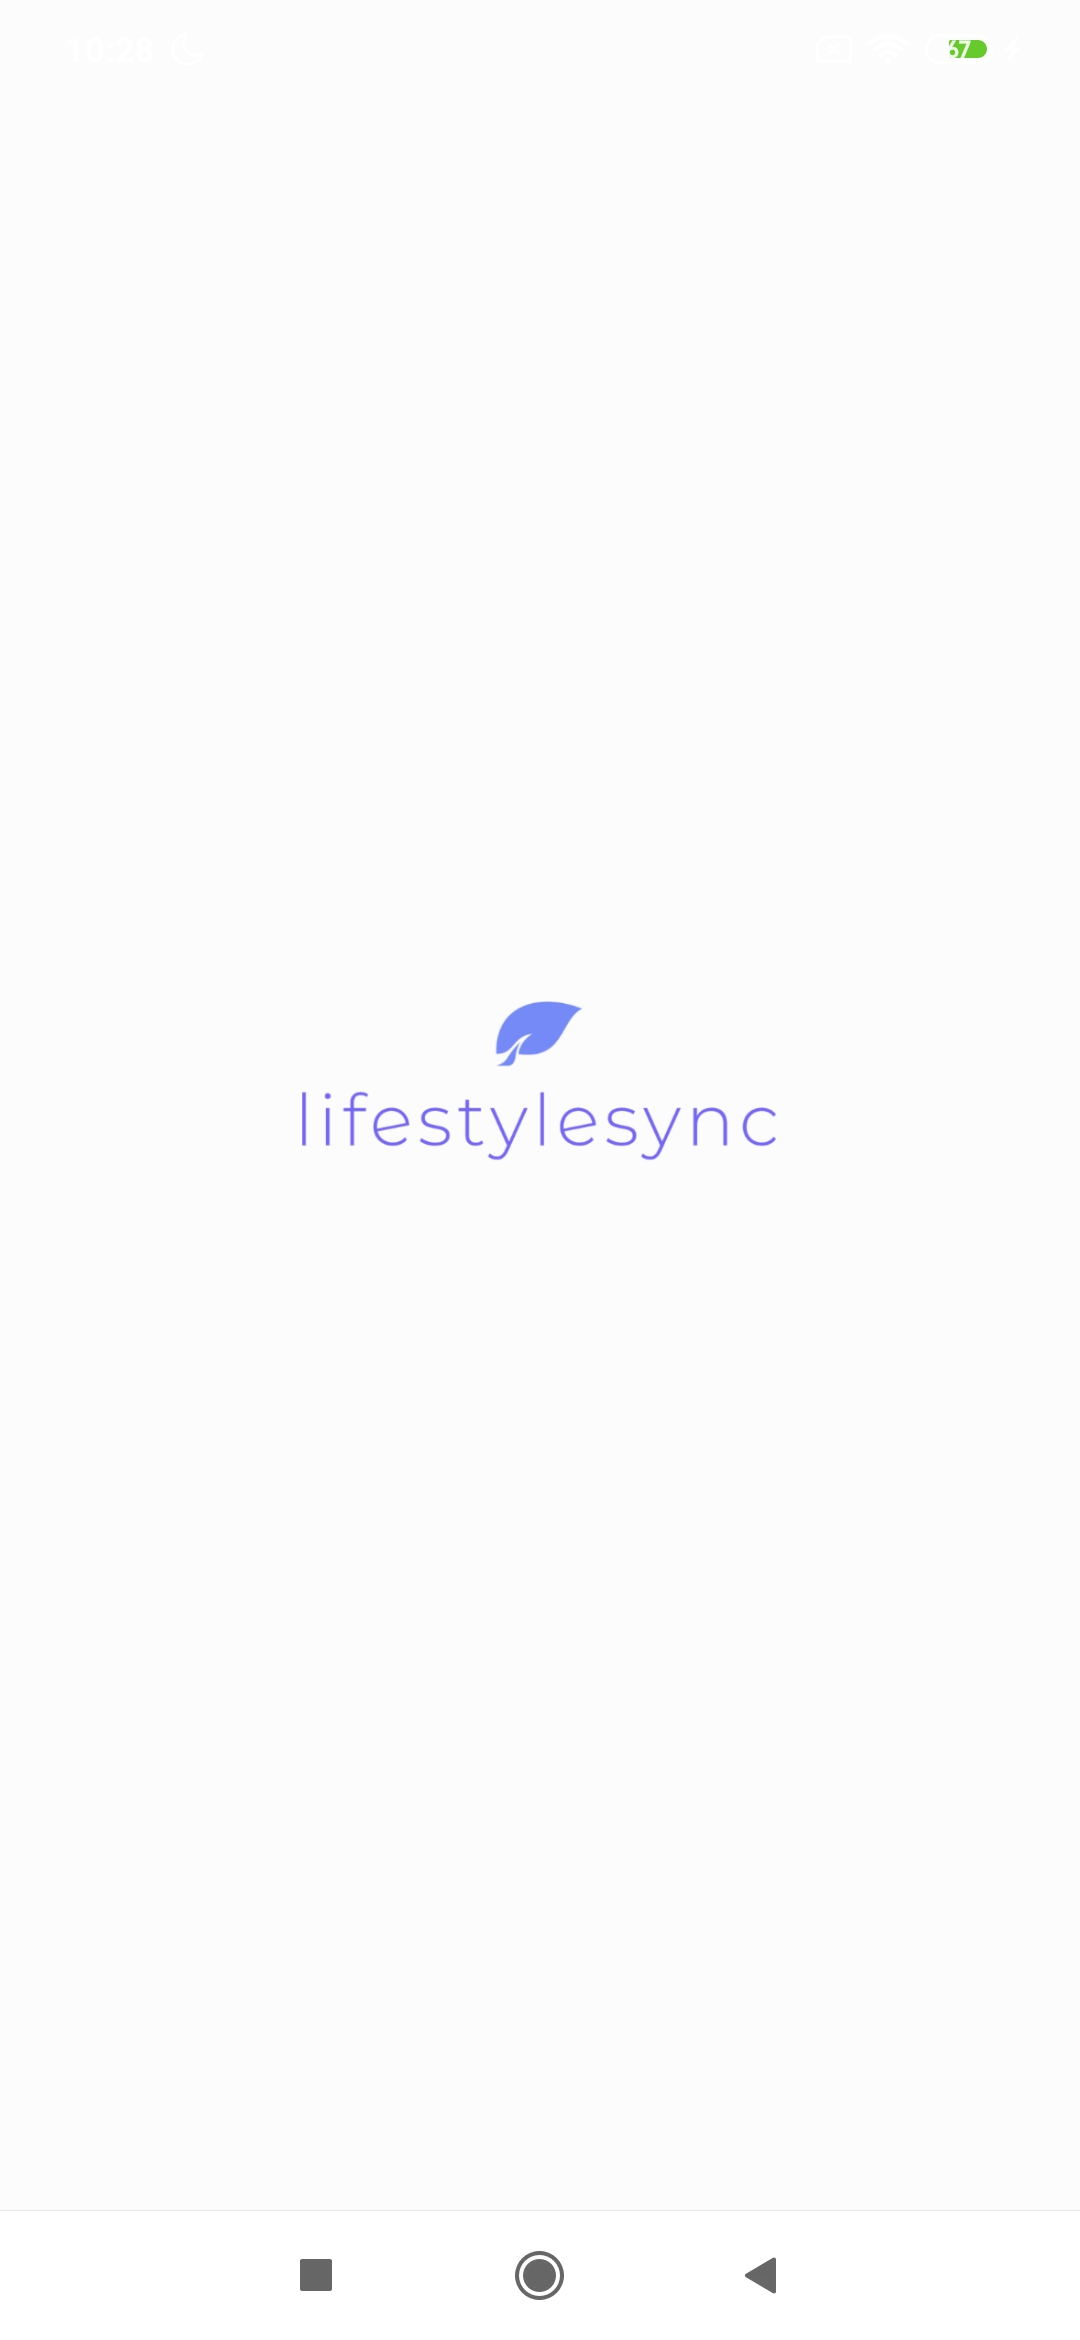
\includegraphics[width = 4cm]{app_screenshot/splash_screen.jpg}} 
\hspace{0.1cm}
\subfloat[Waiter Screen]{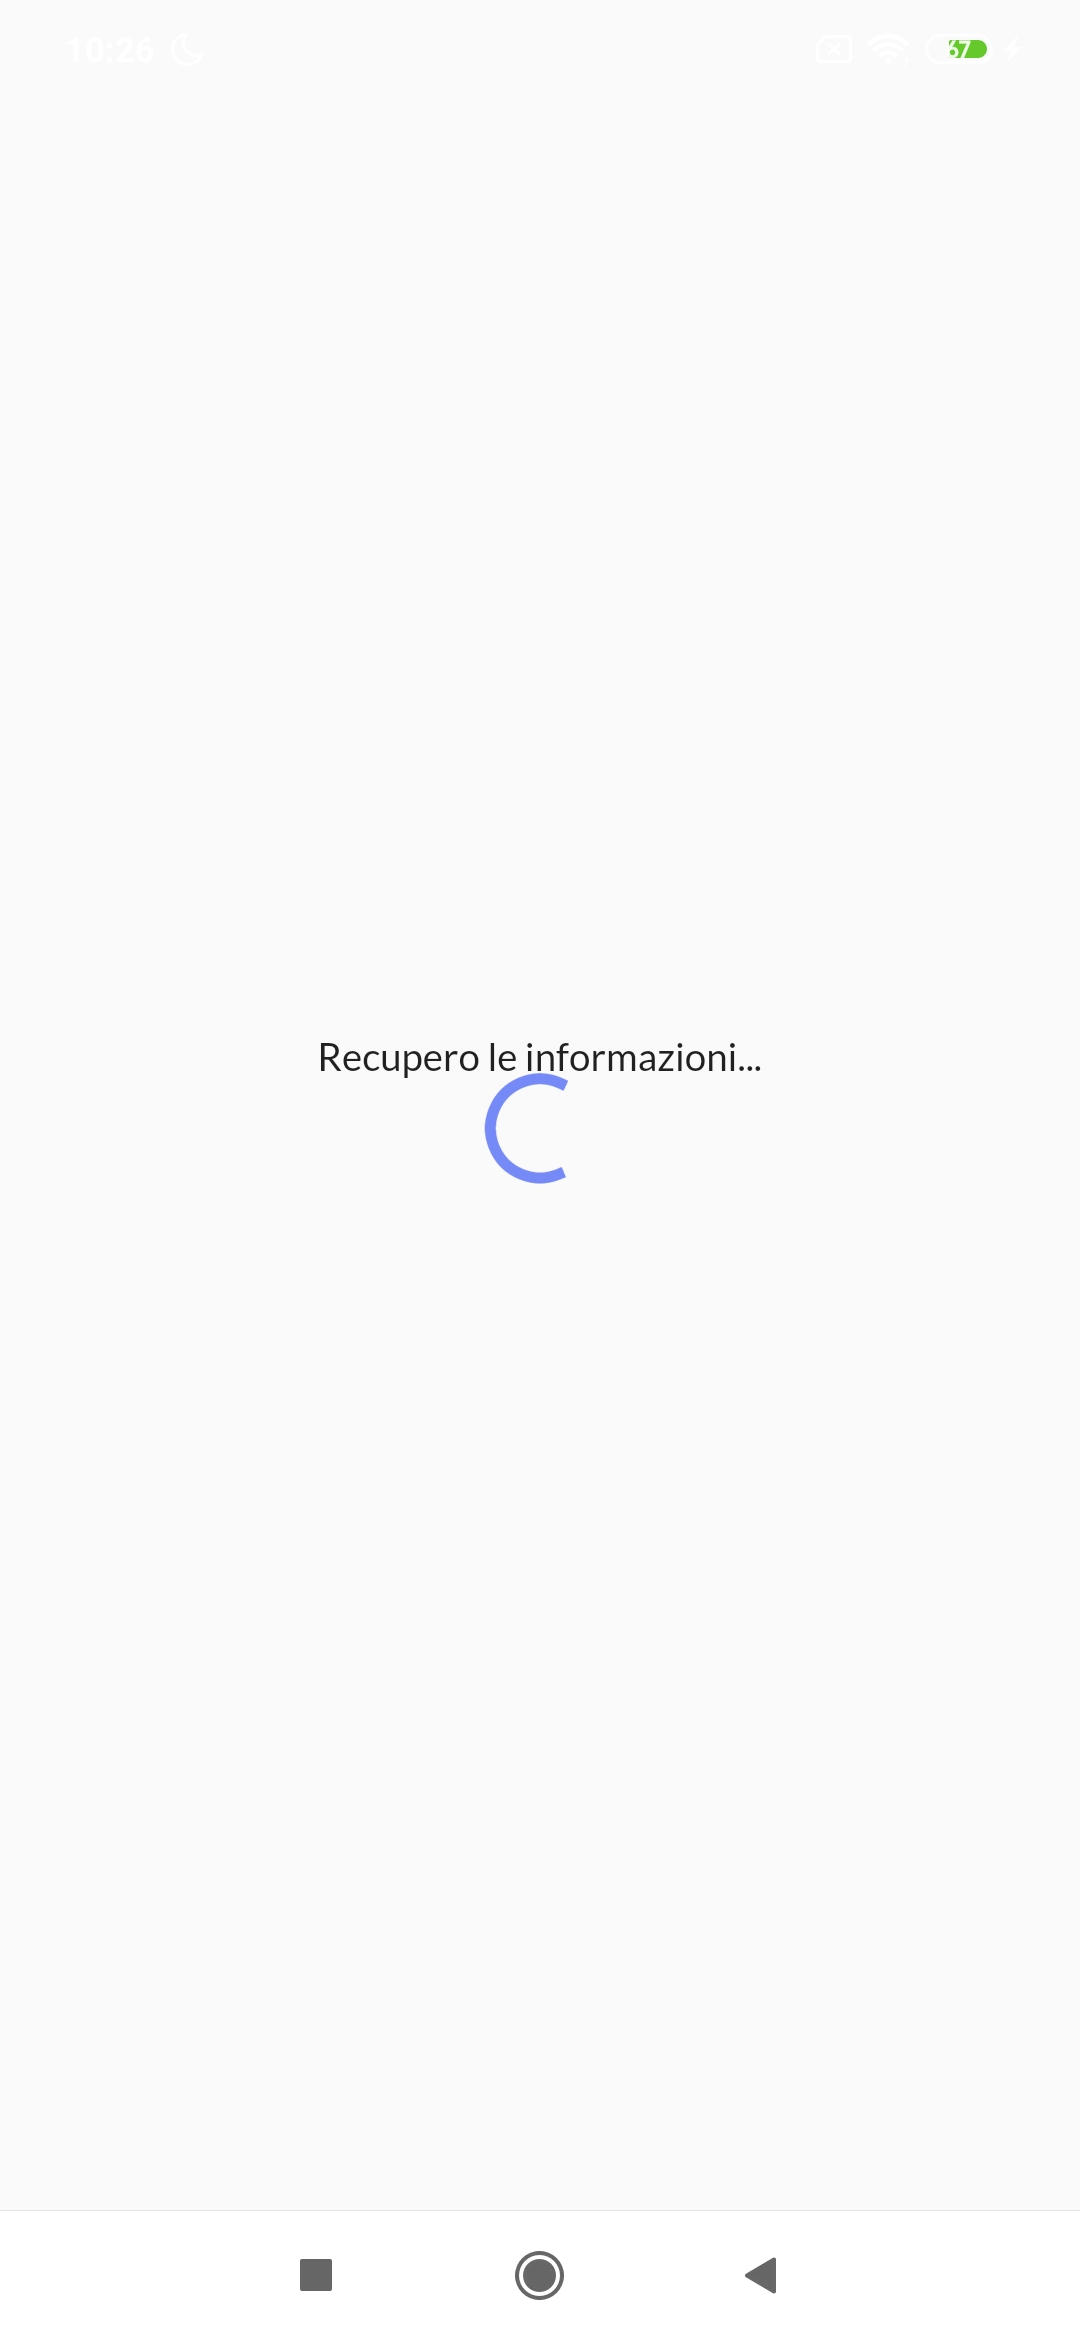
\includegraphics[width = 4cm]{app_screenshot/waiter.jpg}}
\hspace{0.1cm}
\subfloat[Login Screen]{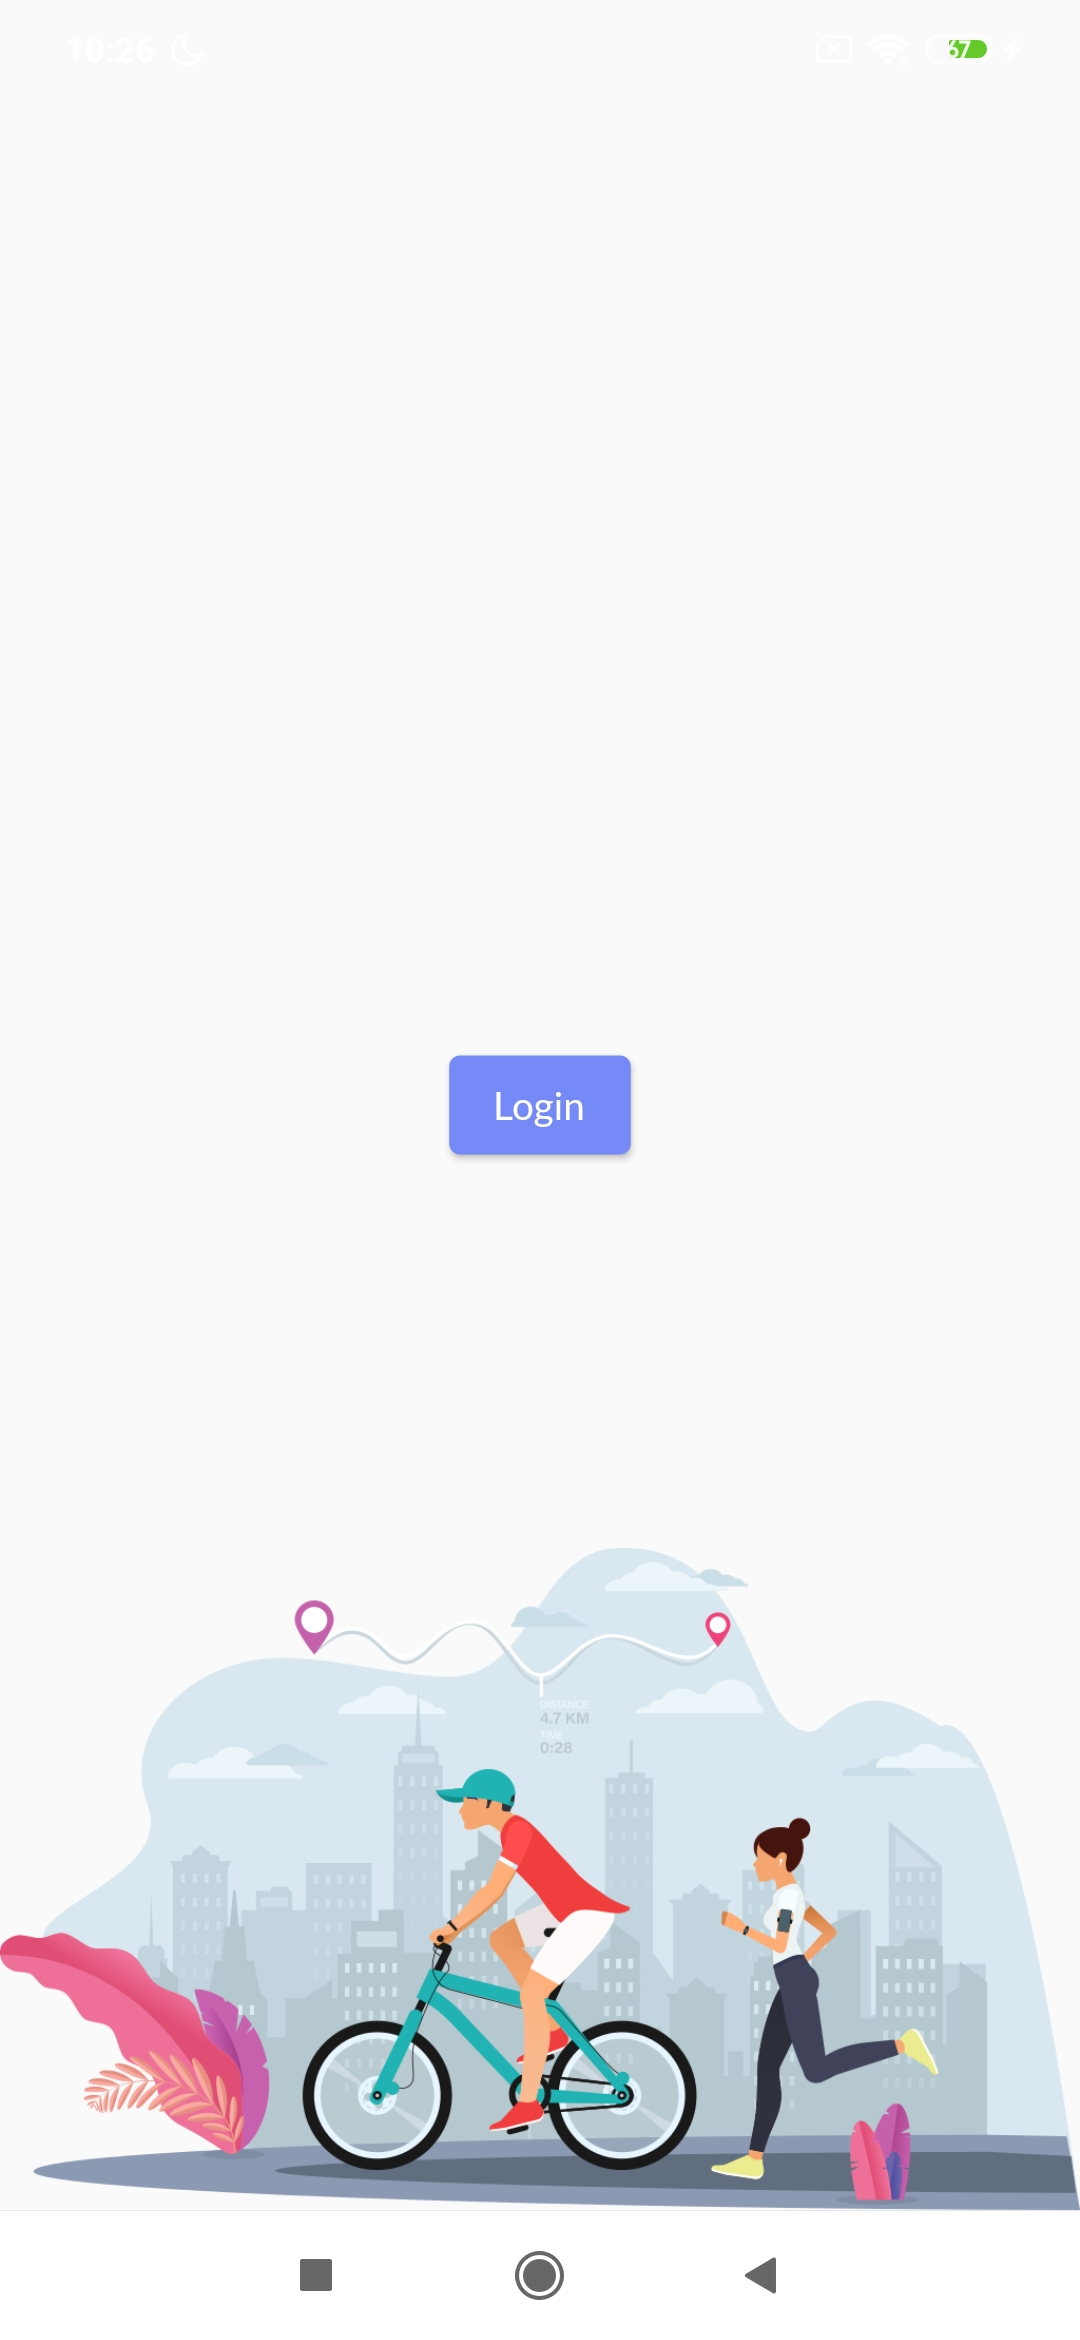
\includegraphics[width = 4cm]{app_screenshot/login.jpg}}
\caption{Prime schermate dell'applicazione}
\end{figure}
\end{center}
%%%%%%%%%%%%%%%%%%%%%%%%%%%%%%%%%%%%%%%%%%%%%%%%%%%%%%%%
A supporto di questi widget sono stati sviluppati tre widget fondamentali:
\begin{itemize}
    \item GenericErrorPage: accetta come parametro un messaggio di errore e presenta all'utente una generica pagina di errore con il messaggio passato come parametro;
    \item Waiter: accetta come parametro un messaggio e presenta all'utente una generica pagina di caricamento con il messaggio passato come parametro;
    \item DelayedWidget: accetta come parametro un numero di secondi ed una condizione da soddisfare. Alla costruzione del widget si avvia un timer della durata dei secondi passati come parametro. Mentre il timer è attivo o la condizione non è soddisfatta si presenta un widget di caricamento, solitamente \textbf{Waiter}, altrimenti viene mostrato all'utente un secondo widget passato anch'esso come parametro. Questo widget è fondamentale per evitare di avere caricamenti talmente brevi da non far vedere all'utente che l'applicazione sta recuperando dei dati.
\end{itemize}
\begin{lstlisting}[language=dart, firstnumber=1,caption={Classe DelayedWidget}]
class DelayedWidget extends HookWidget {
  final Widget child;
  final int timer;
  final bool condition;
  DelayedWidget({
    Key? key,
    required this.child,
    required this.timer,
    required this.condition,
  }) : super(key: key);
  @override
  Widget build(BuildContext context) {
    final timerCondition = useState(false);
    useEffect(() {
      Future.delayed(Duration(seconds: timer))
          .then((value) => timerCondition.value = true);
    }, []);
    if (timerCondition.value && condition)
      return child;
    else
      return Waiter(msg: "Caricamento");
  }
}
\end{lstlisting}

%*************************************************************************
\subsection{ui / ux}
La seguente classe è stata definita per contenere tutti i dati che l'applicazione necessita di conoscere rispetto all'utente che ha effettuato l'accesso. Nel caso dell'applicazione client, esiste una sola unica istanza di \textit{User} e questa viene fornita a qualsiasi widget la necessiti attraverso un provider dedicato.\\
Tale classe si compone di diversi attributi primitivi e di due attributi che sono istanze di altre classi:
\begin{itemize}
    \item \textbf{Info}: contiene le informazioni dell'utente tra cui anche un campo coach, istanza di una classe \textbf{Coach} la quale contiene i dati del proprio coach;
    \item \textbf{Metadata}: contiene i meta-dati dell'utente.
\end{itemize}
\begin{figure}[h]
    \centering
    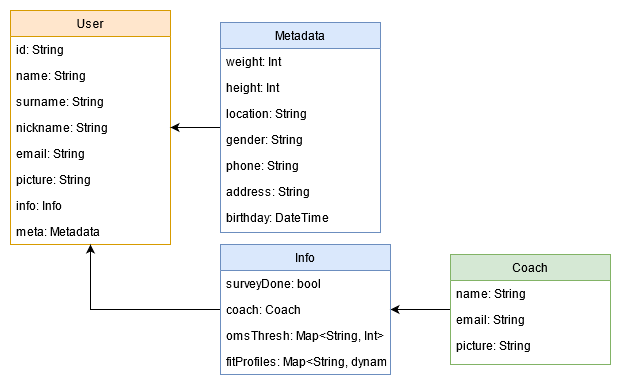
\includegraphics[height=8cm]{user_model}
    \caption{Modello di User}
\end{figure}
\subsection{Introduzione all'app e questionario}
Nel caso in cui sia il primo accesso di un utente, si è deciso di introdurlo all'utilizzo di LifestyleSync attraverso alcune schermate riassuntive delle principali funzionalità dell'applicazione.\\
Come ultima schermata inoltre viene presentato all'utente il coach che gli è stato assegnato, e successivamente gli viene presentato un questionario che è obbligato a compilare per continuare con l'utilizzo dell'applicazione.\\
Al termine del questionario le risposte vengono inviate al backend che si occupa anche di aggiornare le informazioni dell'utente segnando che ha completato il questionario, di conseguenza al prossimo login non dovrà ripeterlo e potrà utilizzare l'applicazione normalmente.\\
Per la realizzazione dei widget del questionario si è deciso di utilizzare una libreria anziché costruire tutte le diverse \textit{form} manualmente. Tra tutte le librerie trovate e provate la migliore si è rivelata \textit{SurveyKit}.\\
\textit{SurveyKit} rende disponibile un buon numero di widget altamente personalizzabili per diversi tipi di domande: risposta singola, multipla, radio button, checkbox, e via dicendo. Inizialmente non si sono presentati problemi nell'utilizzo di tale libreria, ma una volta terminato lo sviluppo si è presentato un bug, il quale porta al \textit{crash} dell`applicazione nel caso in cui l'utente annulli la compilazione del questionario.\\
Lo sviluppatore della libreria ha deciso di assegnare ad un tasto "Annulla" un metodo che va a rimuovere l'ultima pagina caricata nello stack del \textit{Navigator} di Flutter (Widget standard per la gestione del routing in Flutter) senza però controllare che una volta rimossa l'ultima pagina ce ne siano delle altre da presentare.\\
Nel nostro caso il questionario non viene caricato nello stack e di conseguenza, alla rimozione dell'ultima pagina caricata viene rimossa l'unica pagina caricata nello stack e di conseguenza l'applicazione va in errore e termina.\\
Per risolvere tale problema si è reso necessario il \gls{fork} della libreria e la rimozione del tasto "Annulla" dai diversi widget. Questo non risulta un problema in quanto l'utente è obbligato a compilare il questionario per proseguire nell'utilizzo dell'applicazione.\\
Generalmente viene sconsigliato il \gls{fork} di una libreria in quanto si perde la possibilità di mantenerla aggiornata con le future \textit{release}. Nel nostro caso però, avendo effettuato una minima modifica, ci rimane comunque possibile aggiornare la libreria alle future versioni ed eventualmente andare a ritoccare qualche riga di codice.\\
\newpage
%%%%%%%%%%%%%%%%%%%%%%%%%%%%%%%%%%%%%%%%%%%%%%%%%%%%%
\begin{center}
\begin{figure}[H]
\subfloat[Presentazione coach]{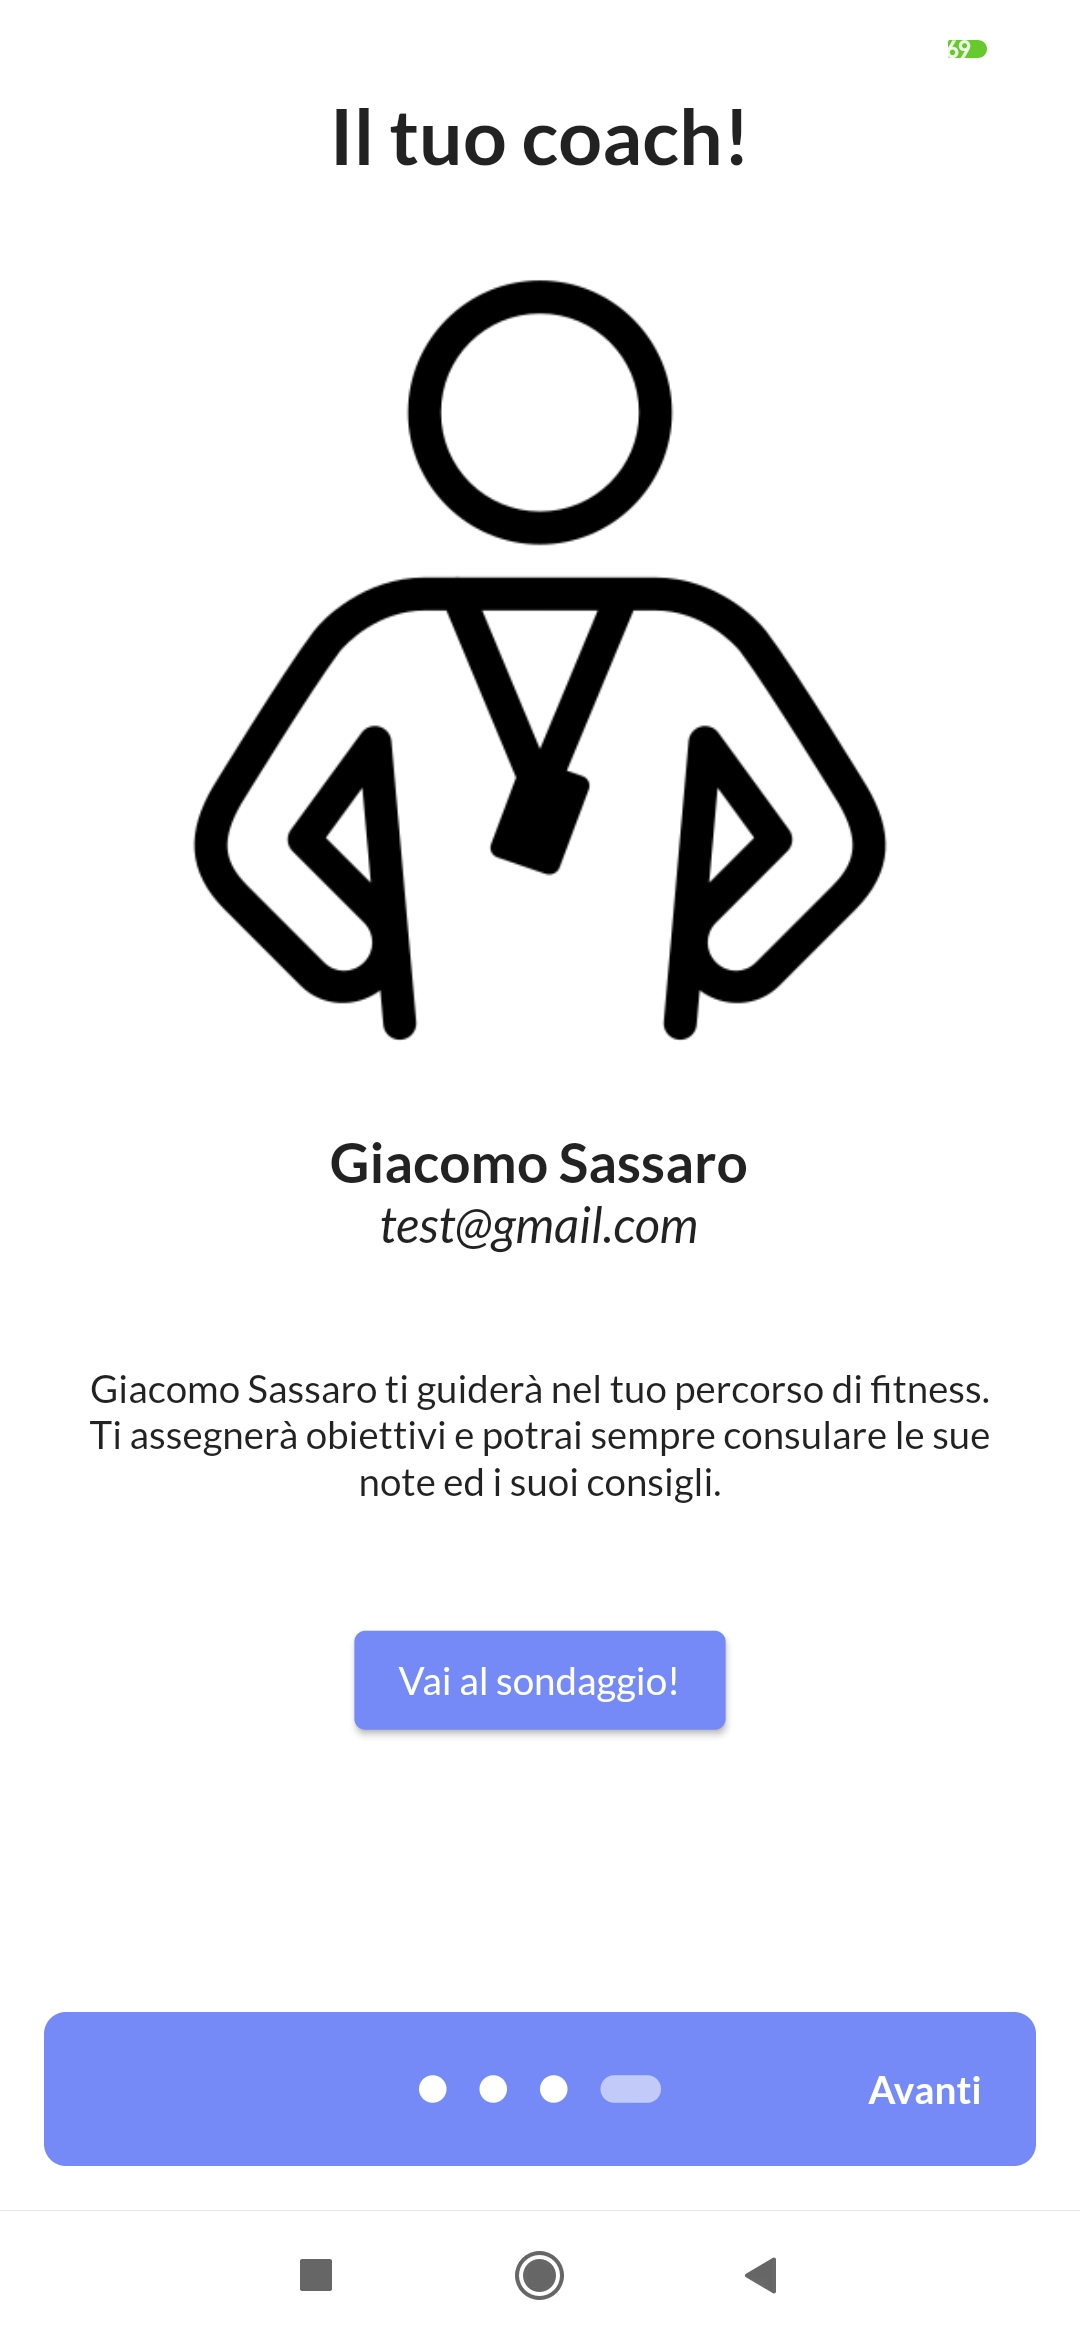
\includegraphics[width = 4cm]{/app_screenshot/coach_info.jpg}} 
\hspace{0.1cm}
\subfloat[Domanda questionario]{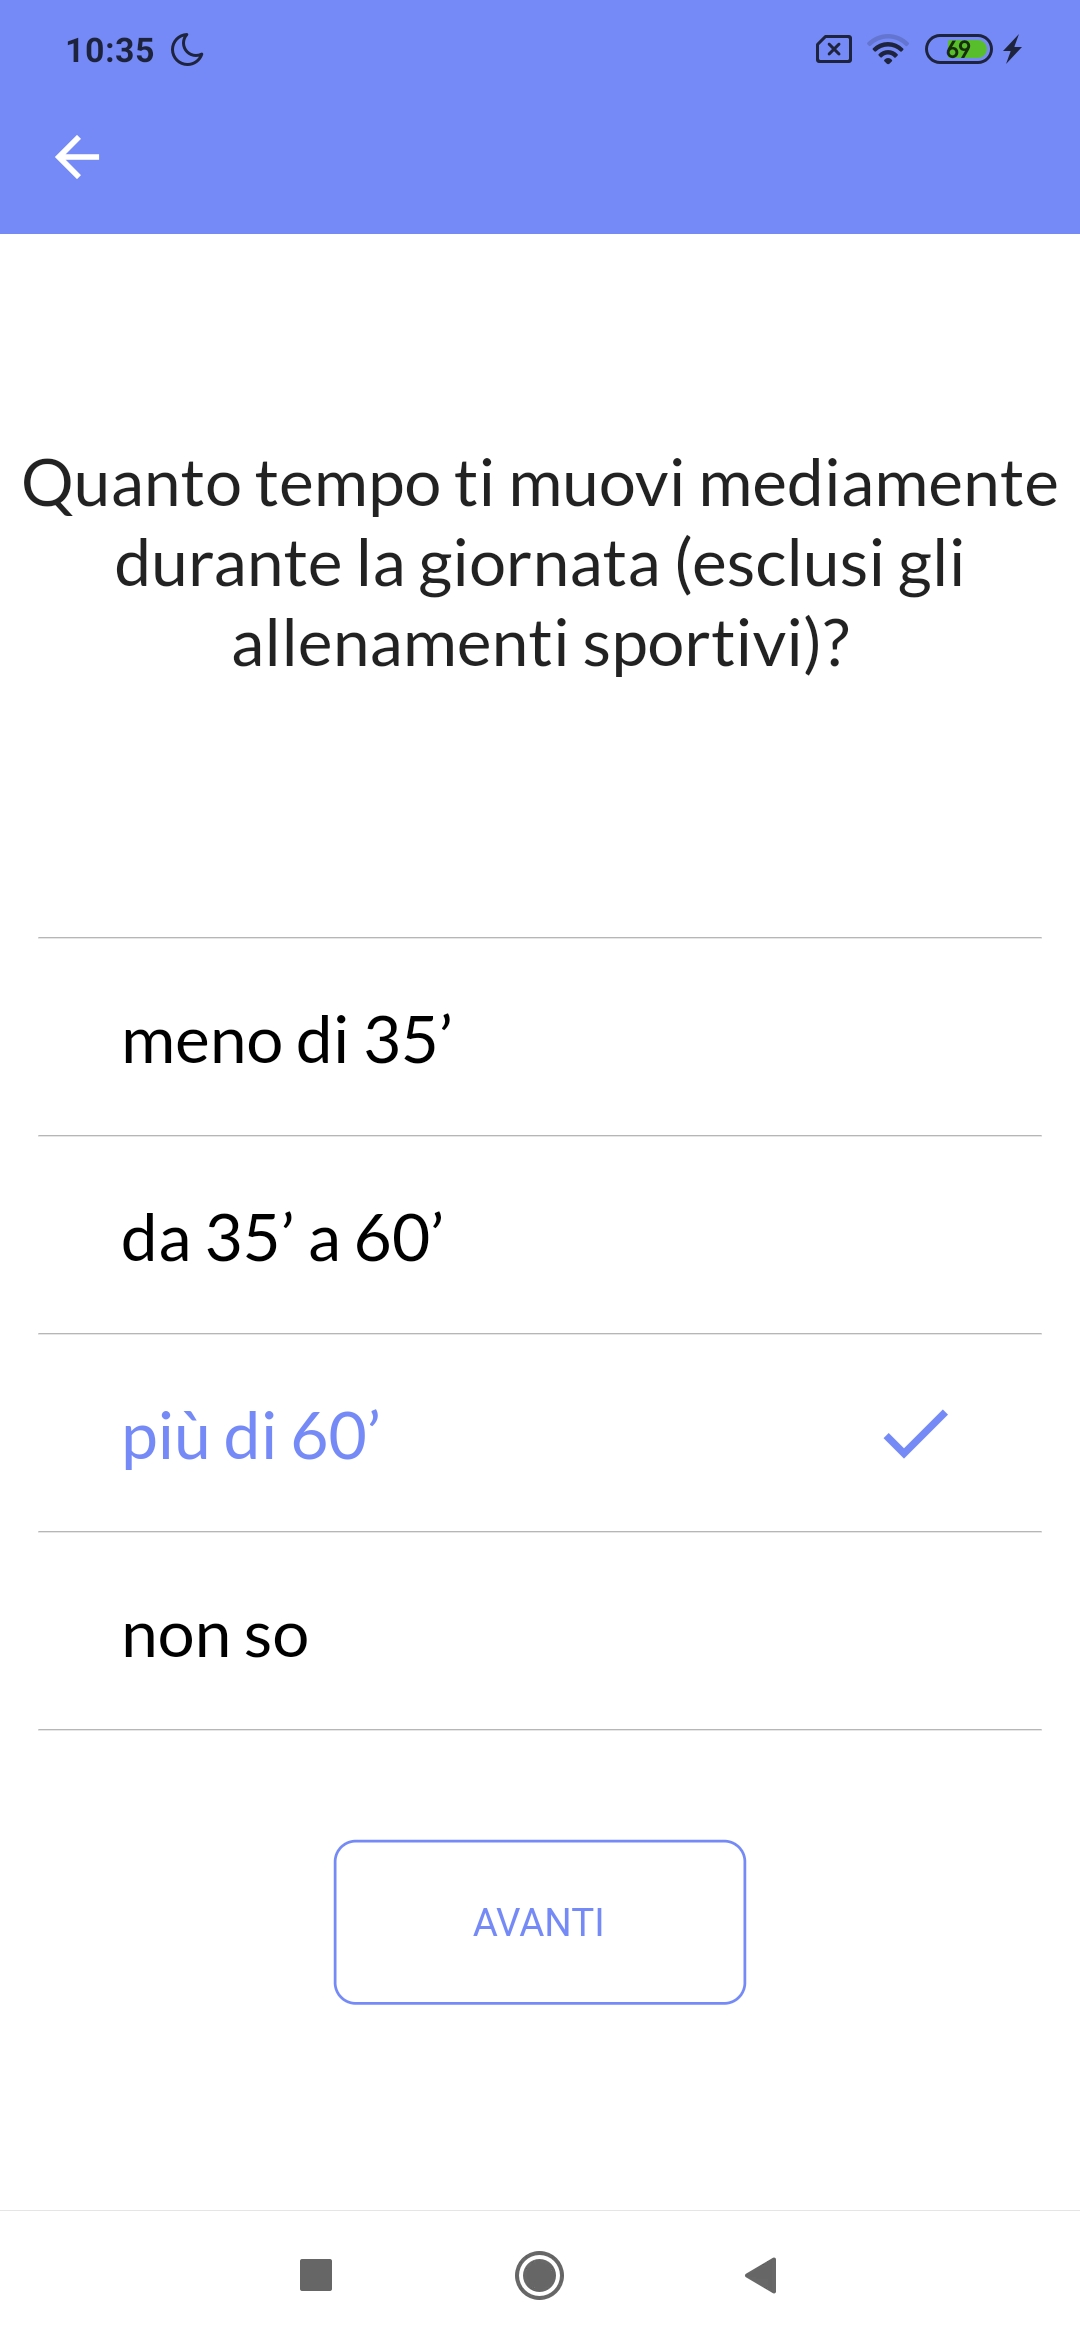
\includegraphics[width = 4cm]{app_screenshot/survey_question.jpg}}
\hspace{0.1cm}
\subfloat[Termine questionario]{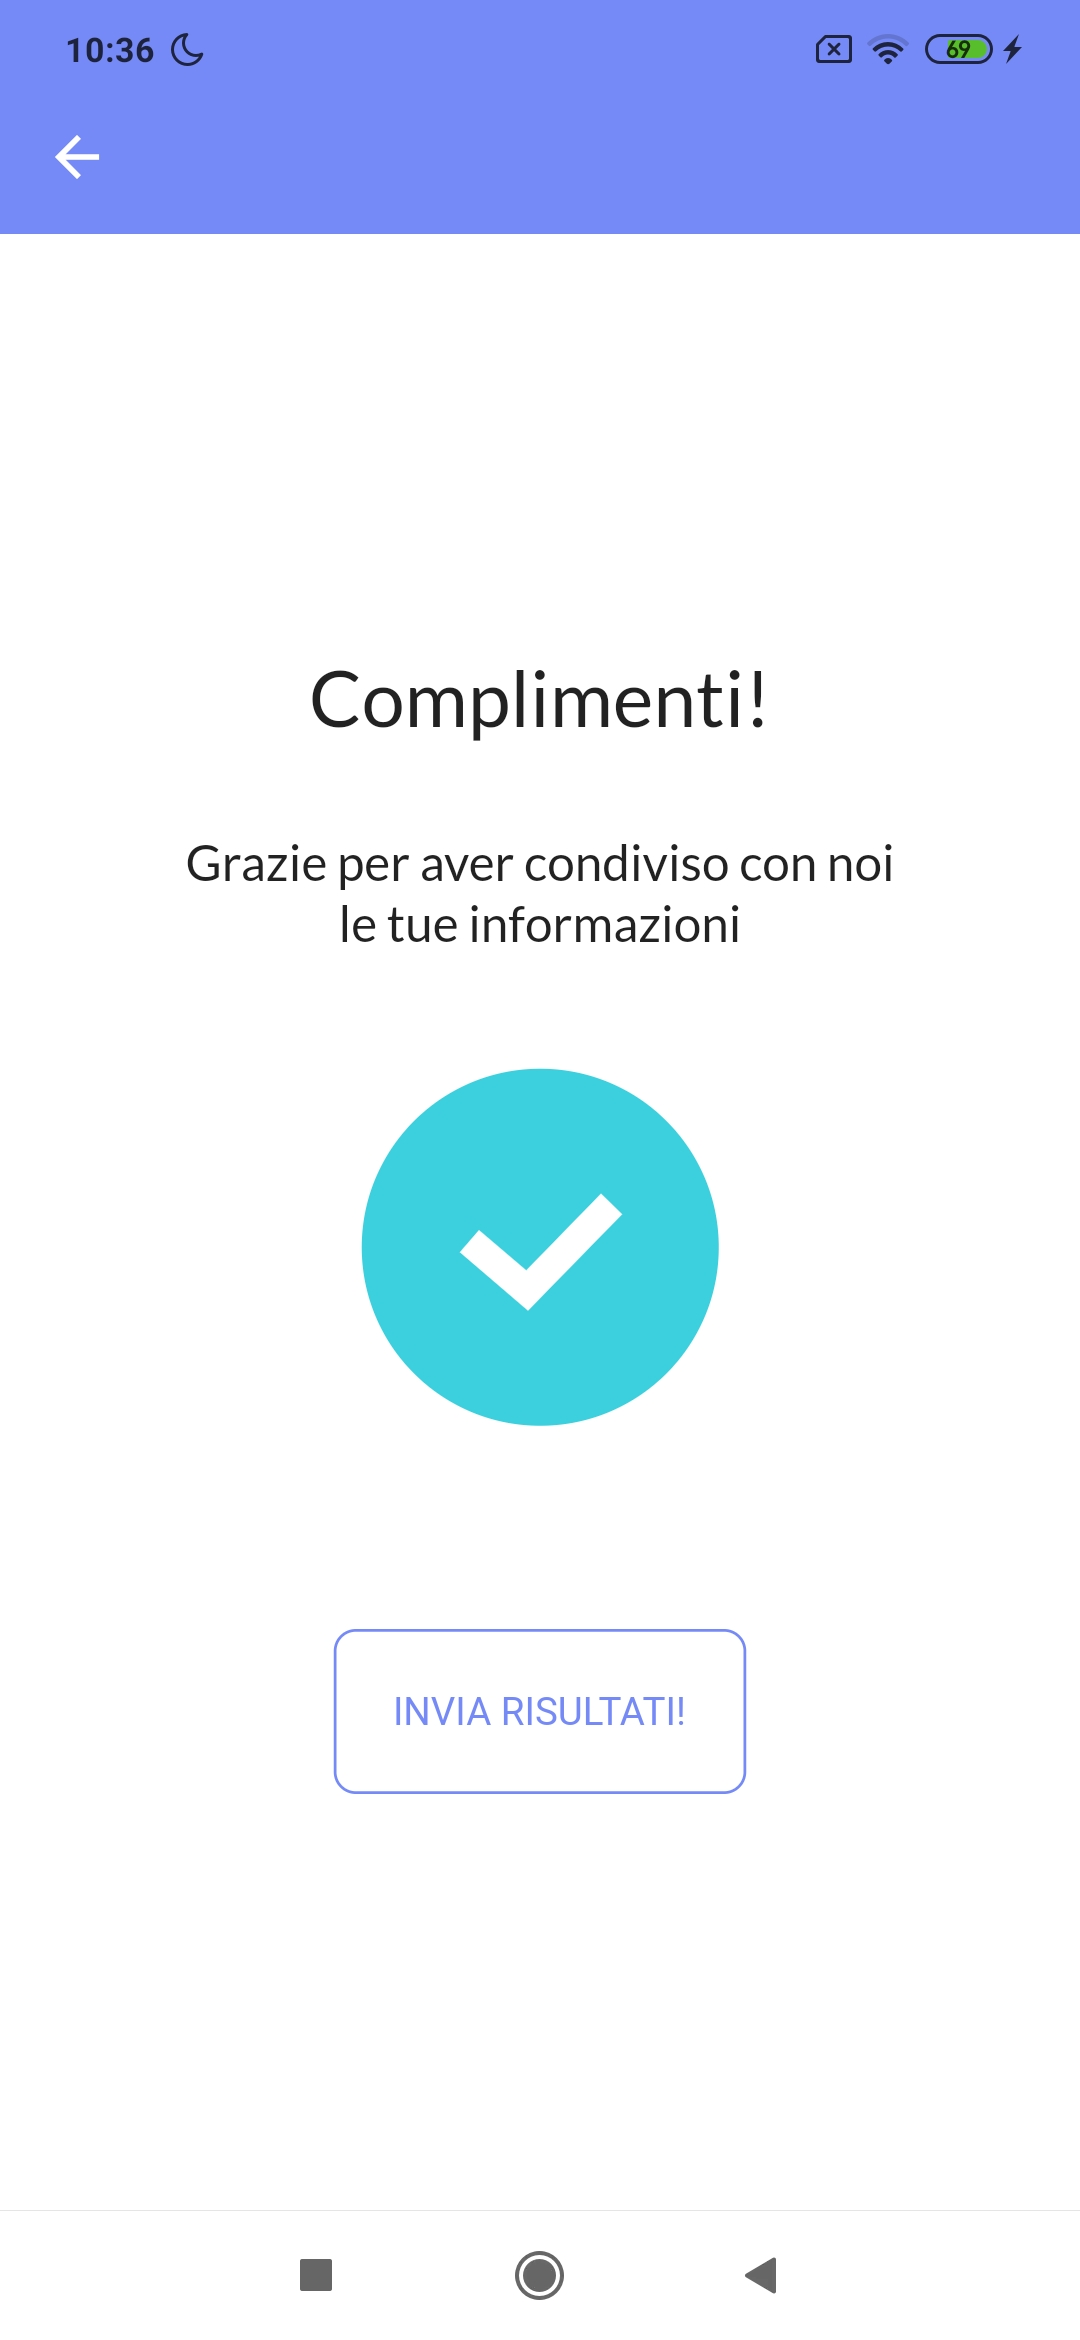
\includegraphics[width = 4cm]{app_screenshot/survey_done.jpg}}
\caption{Alcune schermate onboarding}
\end{figure}
\end{center}
%%%%%%%%%%%%%%%%%%%%%%%%%%%%%%%%%%%%%%%%%%%%%%%%%%%%%
%*************************************************************************
\section{Connessione ai device}
La connessione ai device è stata gestita per la maggior parte dal mio tutor in quanto aveva già utilizzato l'API per l'associazione del profilo LifestyleSync ai profili fitness nel sito web. Il mio compito è stato solamente quello di sviluppare l'interfaccia utente utilizzando i dati che mi venivano restituiti dal provider sviluppato dal mio tutor.\\
In fase di progettazione si pensava di connettere l'applicazione direttamente alle smartband dei diversi produttori (Google Fit, Fitbit, Garmin), in fase di sviluppo però ci si è resi conto che la connessione diretta al dispositivo fisico risultava eccessivamente complessa e si è deciso quindi di associare gli account delle diverse piattaforme di fitness all'account di LifestyleSync, così da prelevare le misurazioni delle smartband dai dati presenti negli account online e non direttamente dal dispositivo fisico.\\
È stata quindi sviluppata una sezione, nella schermata del profilo, attraverso la quale l'utente possa vedere a quali servizi è già connesso e può quindi disconnettersi o viceversa.\\
Nel caso l'utente provi la connessione a un nuovo servizio, premendo nell'apposito pulsante verrà aperta una pagina nel browser dello smartphone in cui è possibile effettuare l'accesso al servizio in questione e autorizzarne il prelievo dei dati. Nel caso in cui l'associazione vada a buon fine viene visualizzato un messaggio di successo e i dati iniziano ad essere salvati nel nostro backend, altrimenti viene visualizzato un messaggio di errore ed è necessario riprovare l'associazione.
\begin{figure}[H]
    \centering
    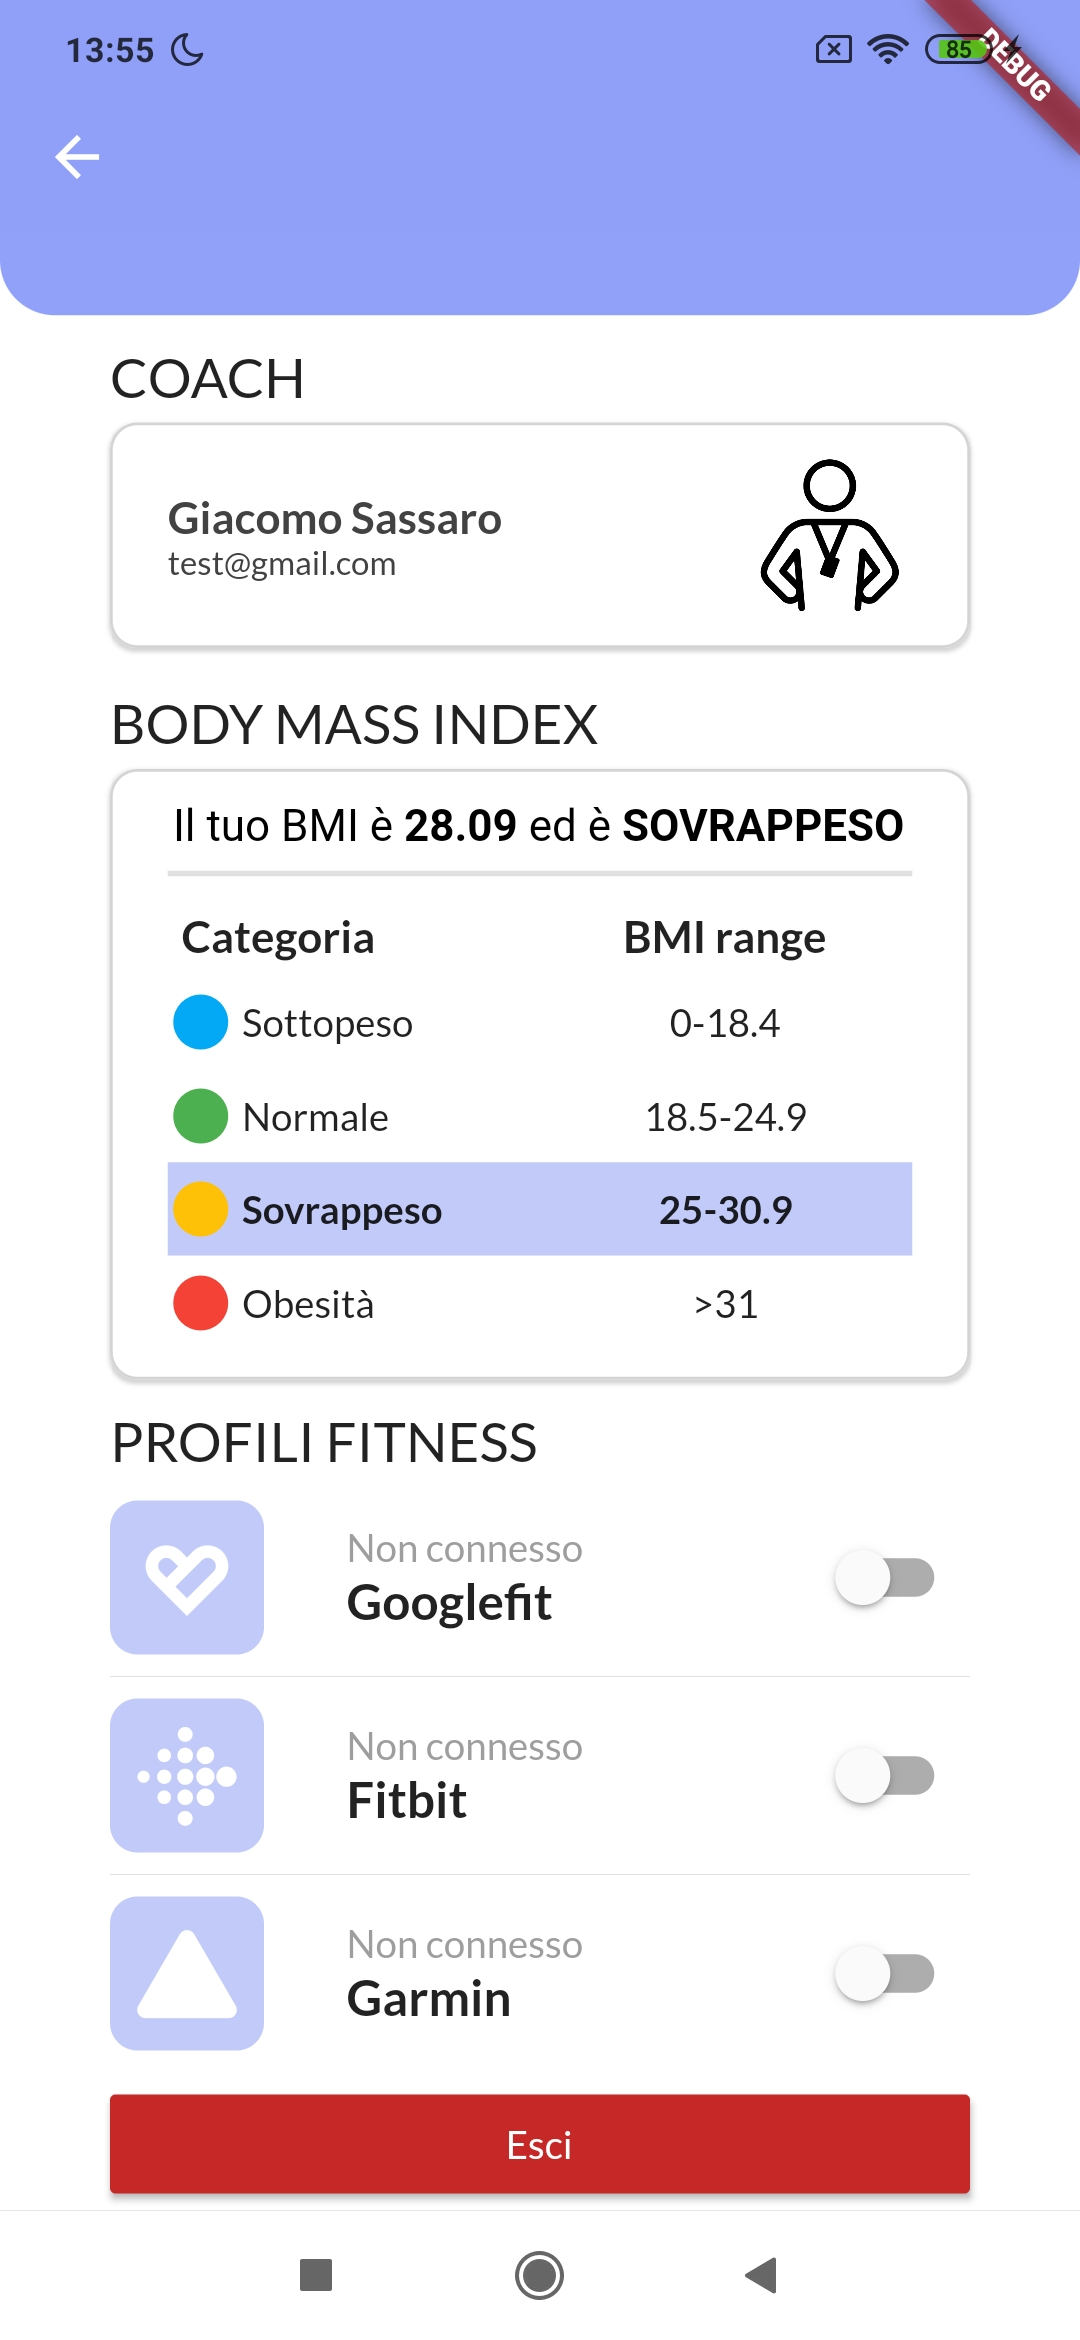
\includegraphics[width=4cm]{app_screenshot/profile_client.jpg}
    \caption{Schermata del profilo cliente con sezione relativa ai profili fitness}
\end{figure}
%*************************************************************************
\section{Dashboard utente}
Una volta completato lo sviluppo delle funzionalità Onboarding si è progredito con lo sviluppo della dashboard utente, ossia delle schermate principali con cui l'utente interagisce durante l'uso quotidiano dell'applicazione.
\subsection{Models}
Nelle varie schermate di dashboard utente sono visualizzati i diversi dati relativi a Obiettivi, Appuntamenti, Risultati e Attività. Tutti questi dati vengono richiesti al backend al caricamento dell'applicazione o nelle schermate che ne fanno uso, questo in base alla scelta progettuale di dove salvare i dati ricevuti: nello store globale o nello store locale di un widget.\\
Per memorizzare tali dati si sono dunque rese necessarie diverse classi: \textit{Goals}, \textit{Appointment}, \textit{Achievement}, \textit{Duration}
Siccome sia \textit{Appointment} che \textit{Goals} possiedono una data di inizio e una di fine, si è deciso di sviluppare una classe astratta \textit{Event} da cui farle ereditare. Questa scelta è stata fatta anche per permettere una scalabilità all'applicazione in quanto in futuro saranno sviluppate altre classi che avranno data di inizio e fine e potranno quindi anche loro ereditare da \textit{Event}.
\paragraph{Event}
Classe astratta rappresentate un evento generico.
\begin{itemize}
    \item \textbf{id}: identificativo dell'evento;
    \item \textbf{start}: data di inizio;
    \item \textbf{end}: data di fine.
\end{itemize}
\paragraph{Goals}
Insieme di obiettivi, questo insieme può essere attivo o passato e può essere stato raggiunto o meno. Attualmente un \textit{Goals} si compone di quattro \textit{Goal}: passi, minuti di attività, minuti non programmati, calorie.
\begin{itemize}
    \item \textbf{goals}: lista di \textit{Goal} indicizzata (steps, durationA, durationN, calories);
    \item \textbf{achieved}: obiettivo completato o meno;
    \item \textbf{active}: obiettivo attivo o meno;
\end{itemize}
\paragraph{Goal}
Un obiettivo da raggiungere che può essere: passi, minuti di attività, minuti non programmati, calorie.
\begin{itemize}
    \item \textbf{metric}: metrica di rilevazione;
    \item \textbf{thresh}: valore da raggiungere;
    \item \textbf{status}: valore attualmente raggiunto;
\end{itemize}
\paragraph{Appointment}
Rappresenta un appuntamento tra un \textit{Coach} e un \textit{Client}.
\begin{itemize}
    \item \textbf{subject}: titolo dell'appuntamento;
    \item \textbf{tenant}: gruppo di clienti al quale appartiene l'appuntamento;
    \item \textbf{notes}: appunti lasciati dal coach;
    \item \textbf{coach}: coach che partecipa all'appuntamento;
    \item \textbf{client}: cliente che partecipa all'appuntamento.
\end{itemize}
\paragraph{Duration}
Minuti di movimento di una giornata.
\begin{itemize}
    \item \textbf{id}: identificativo;
    \item \textbf{duration}: somma di durationA e durationN;
    \item \textbf{durationA}: minuti di attività giornalieri;
    \item \textbf{durationN}: minuti non programmati giornalieri;
    \item \textbf{ts}: data della rilevazione.
\end{itemize}
\begin{figure}[H]
    \centering
    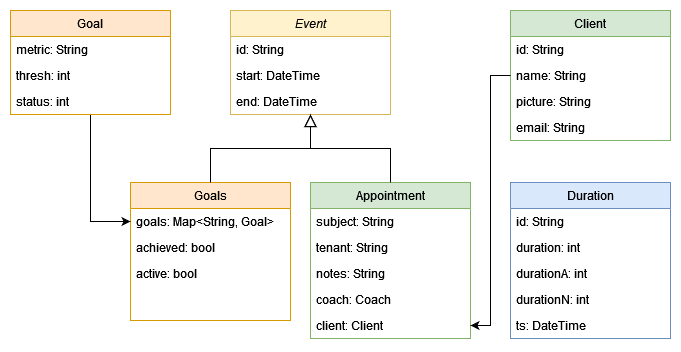
\includegraphics[width=14cm]{models.png}
    \caption{Modelli dei dati}
\end{figure}
\subsection{Homepage}
Una volta predisposti i diversi modelli si sono sviluppati i widget per la rappresentazione di tali dati nell'homepage. Si è deciso di dare un resoconto di quasi tutti i dati nell'homepage, quindi mostrare tramite una card i minuti di movimento (durations), una lista di card con gli obiettivi (goals) e una lista di card con gli appuntamenti (appointment). \\
Da questa schermata l'utente può approfondire tutti i diversi ambiti cliccando su degli appositi widget. Cliccando sul proprio nome l'utente può vedere i dettagli del suo profilo, cliccando sul pulsante "Vedi tutti" di Obiettivi può visualizzare tutto il suo storico di obiettivi, ossia la sezione \textit{Move}, inoltre cliccando su una qualsiasi card può vedere i dettagli dell'evento premuto sia nel caso di un obiettivo sia nel caso di un appuntamento.
%%%%%%%%%%%%%%%%%%%%%%%%%%%%%%%%%%%%%%%%%%%%%%%%%%%%%
\begin{center}
\begin{figure}[H]
\subfloat[Homepage]{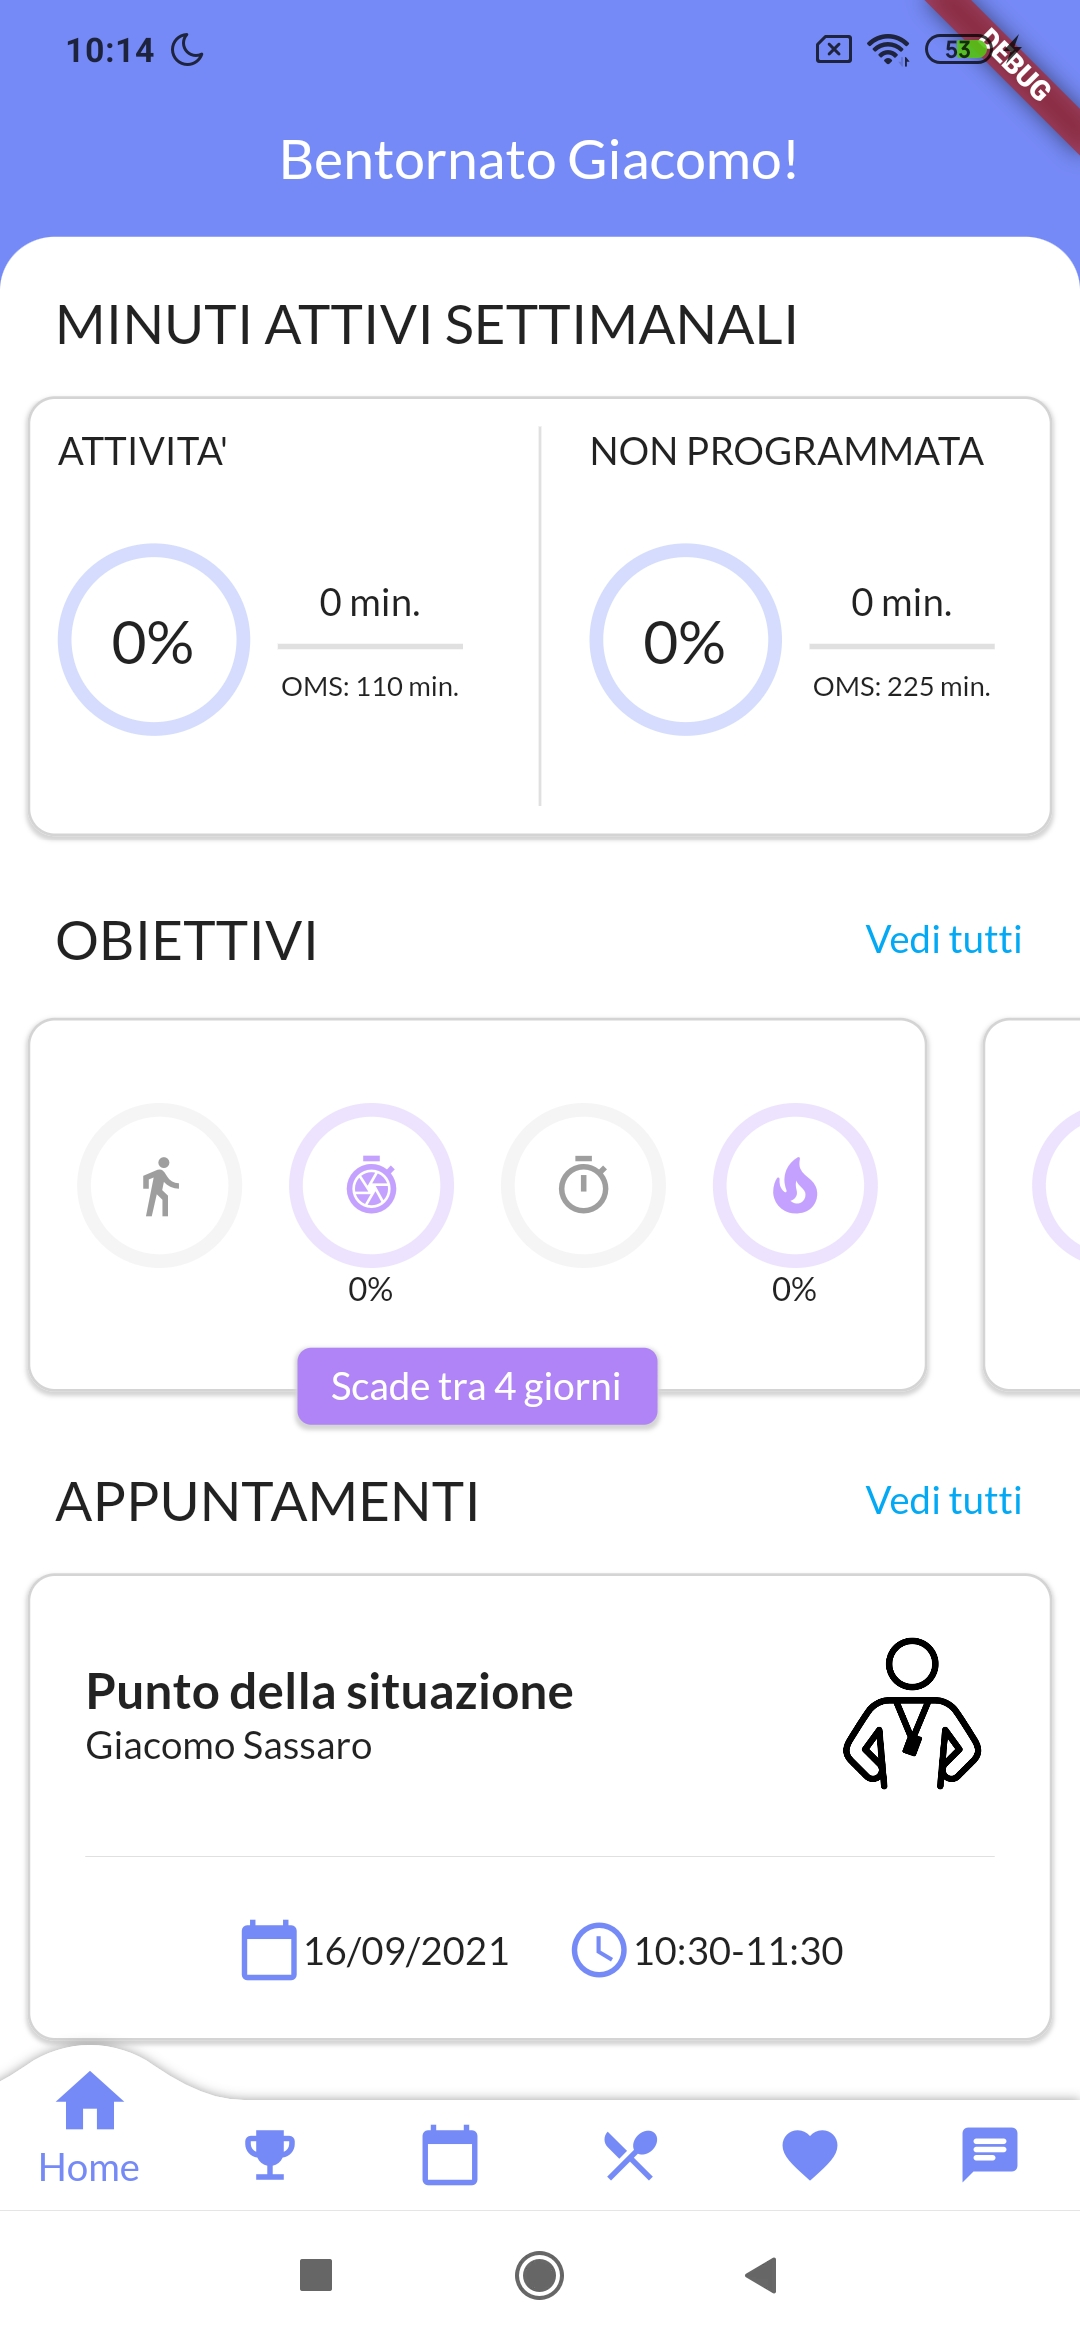
\includegraphics[width = 4cm]{immagini/app_screenshot/homepage_client.jpg}} 
\hspace{0.1cm}
\subfloat[Dettaglio obiettivo]{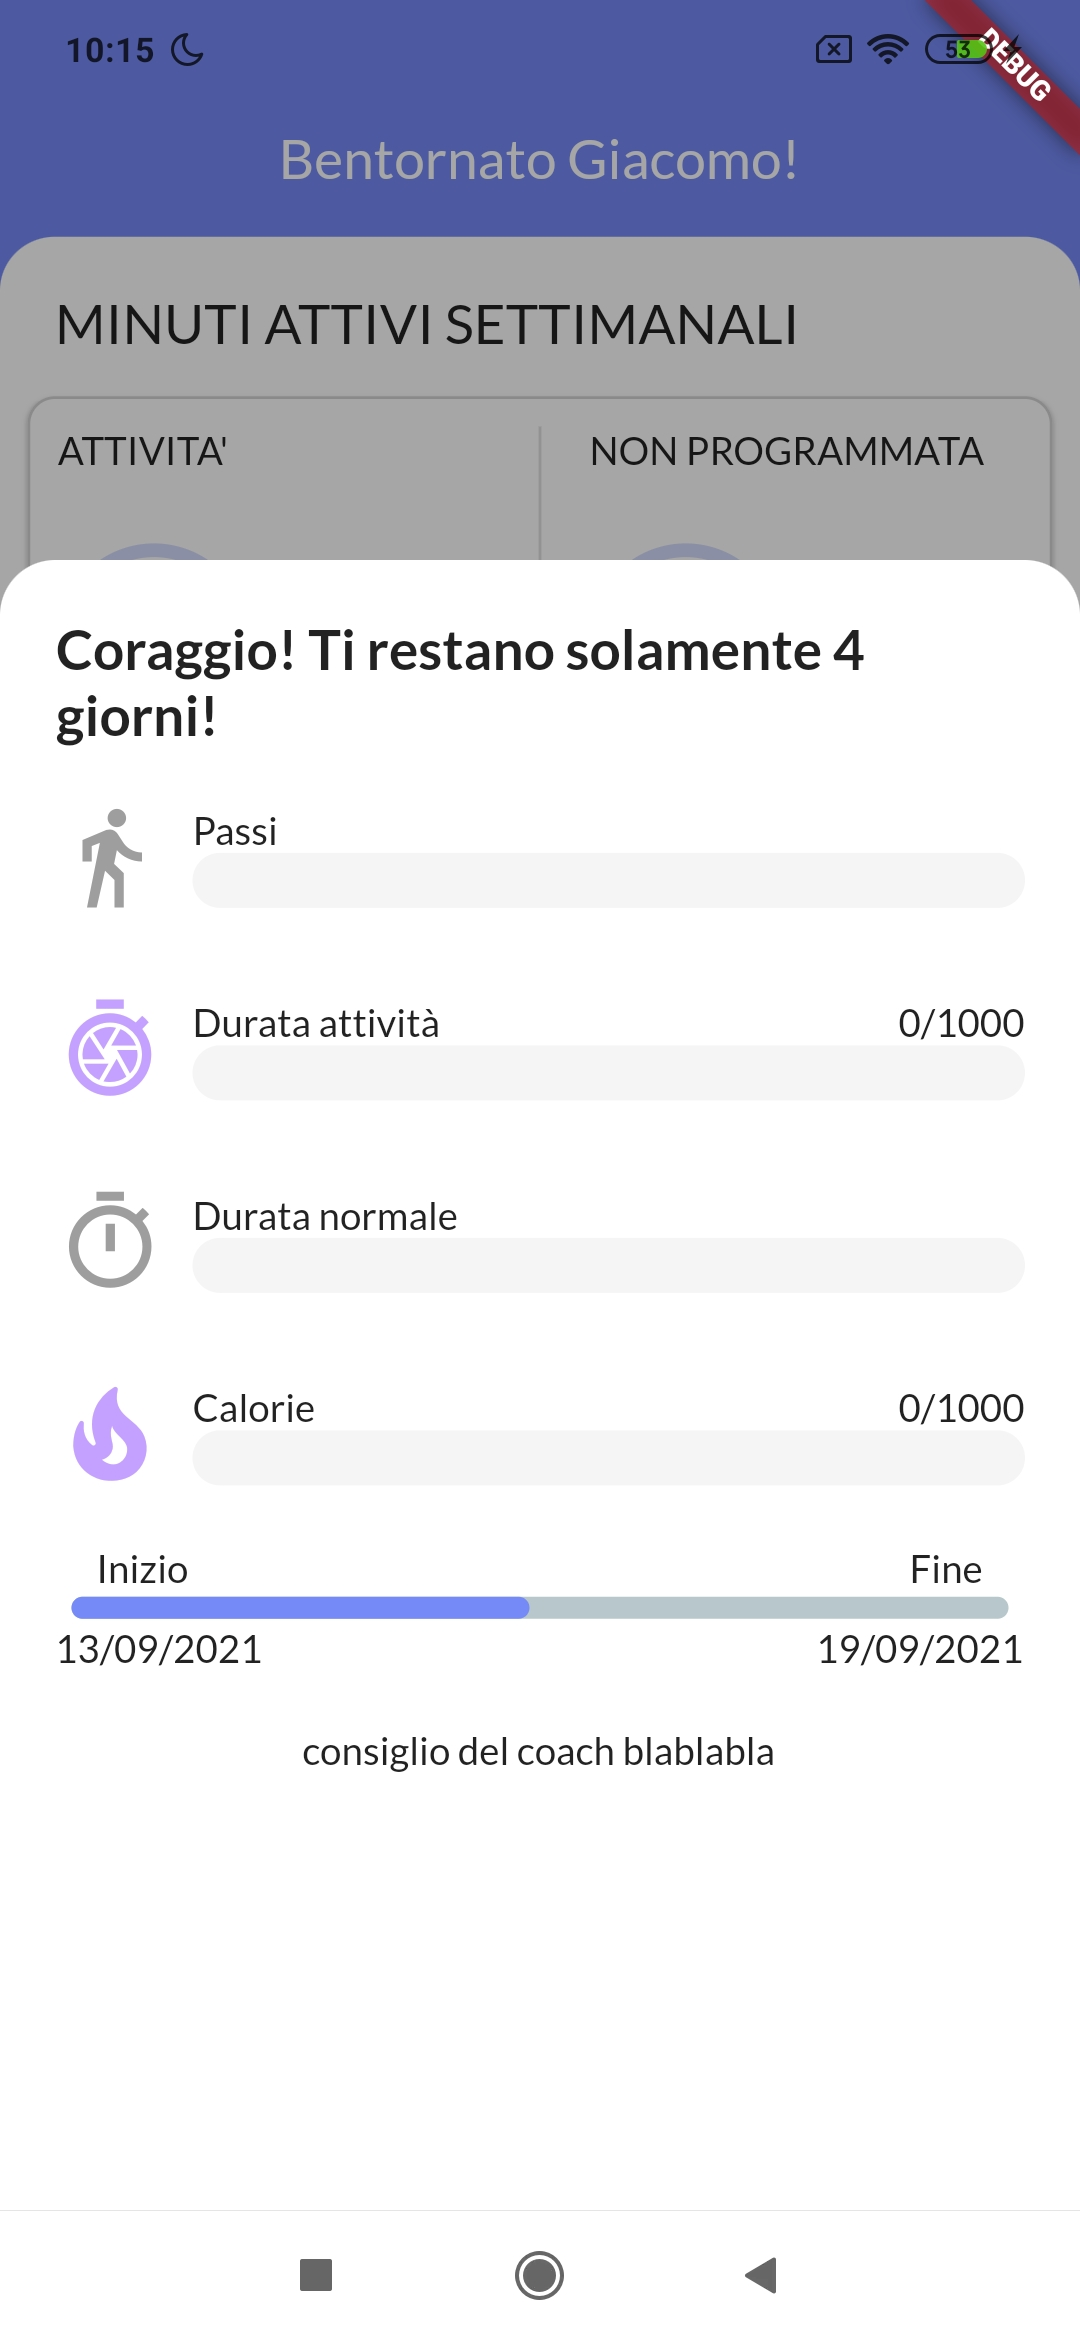
\includegraphics[width = 4cm]{immagini/app_screenshot/goals_details.jpg}}
\hspace{0.1cm}
\subfloat[Dettaglio appuntamento]{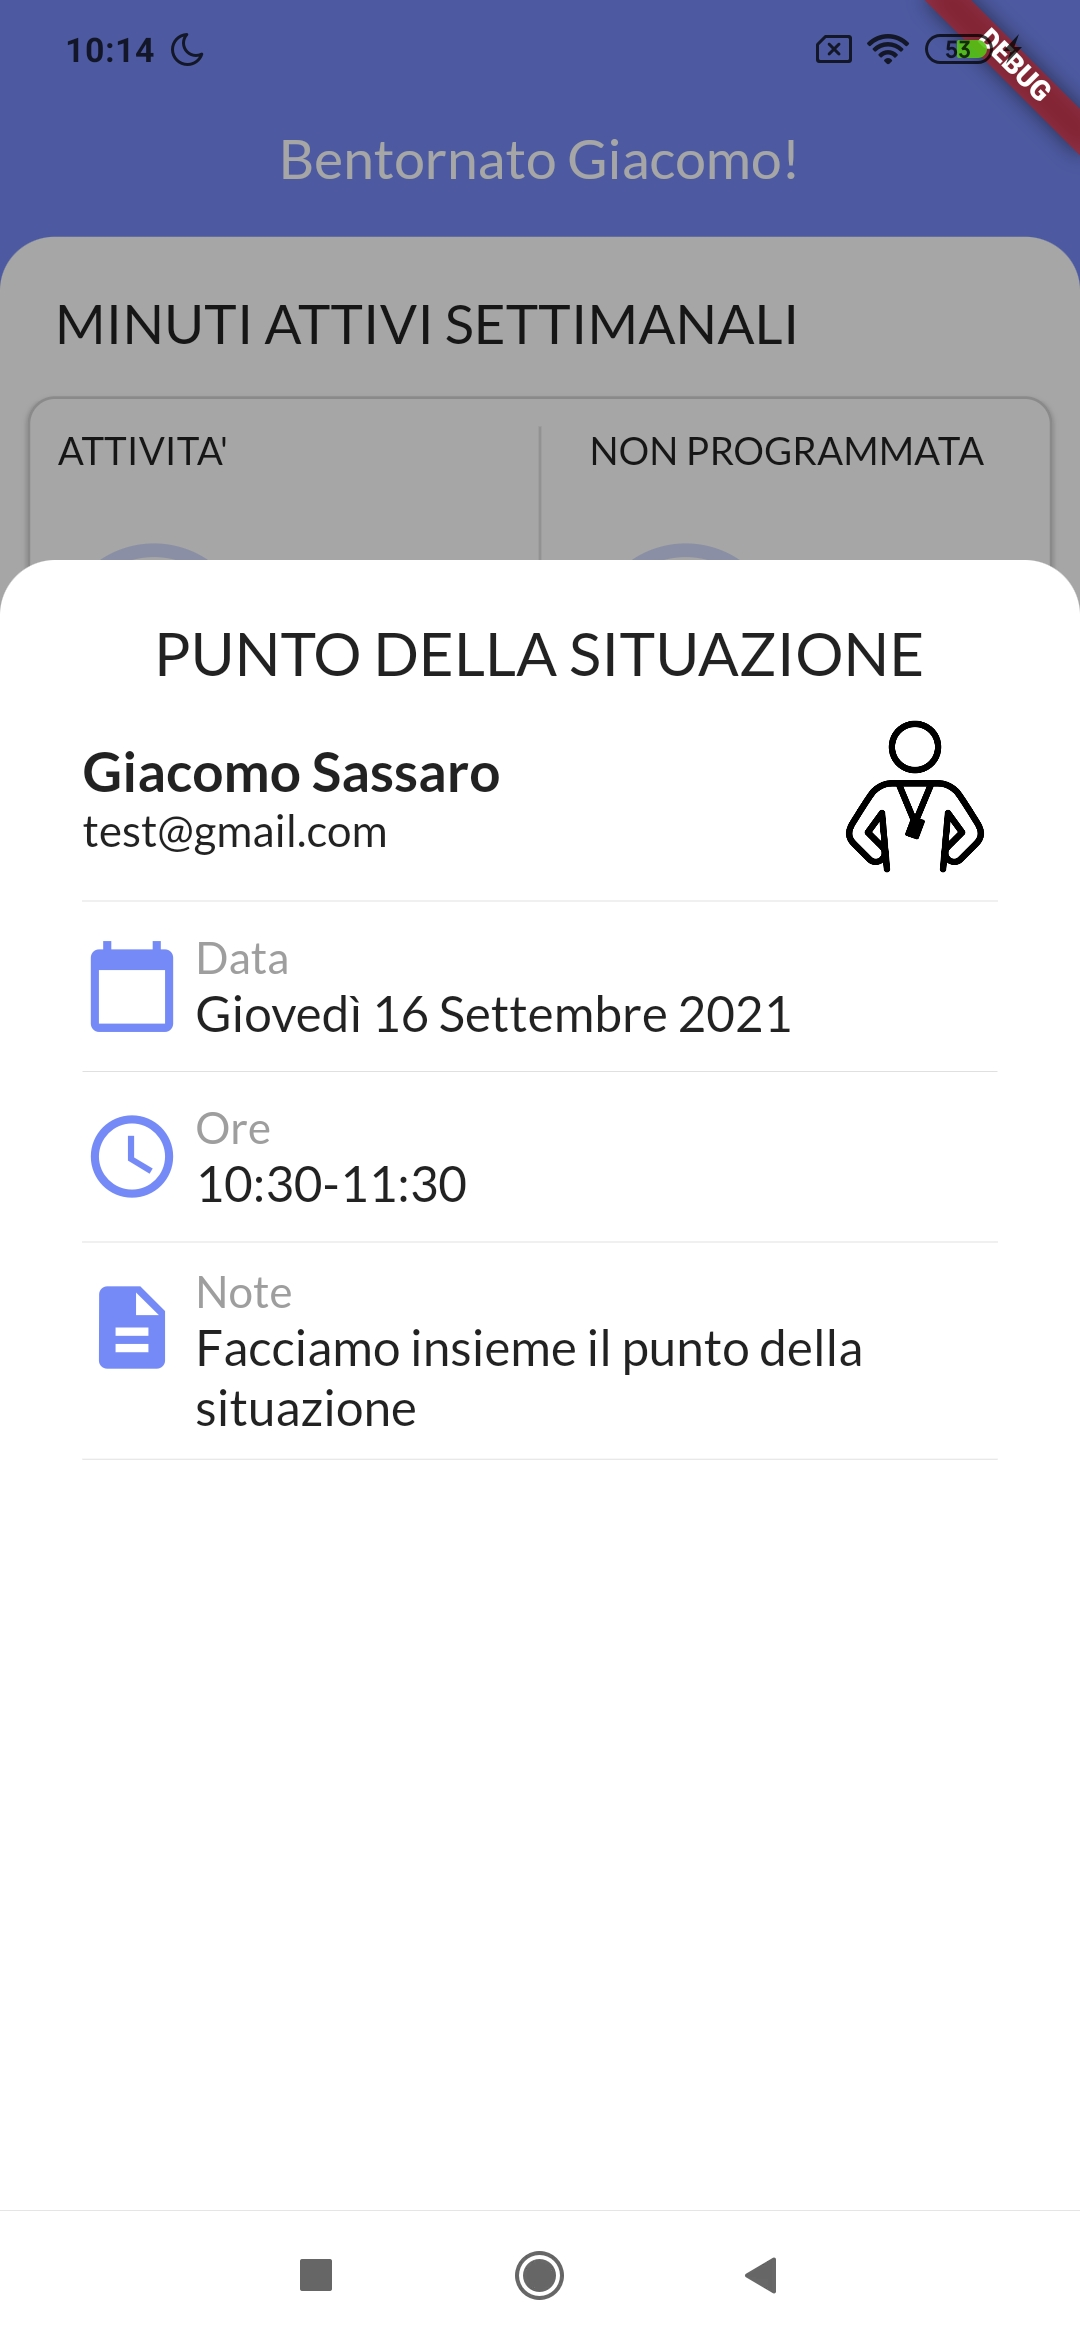
\includegraphics[width = 4cm]{immagini/app_screenshot/appointment_details.jpg}}
\caption{Homepage e dettagli eventi}
\end{figure}
\end{center}
%%%%%%%%%%%%%%%%%%%%%%%%%%%%%%%%%%%%%%%%%%%%%%%%%%%%%
\subsection{Move}
Questa schermata è raggiungibile dalla barra di navigazione o cliccando sul pulsante "Vedi tutti" degli obiettivi nella \textit{Homepage}. Qui si è deciso di presentare all'utente la lista di tutti gli obiettivi attivi, la lista degli obiettivi passati e una sezione con i risultati raggiunti e da raggiungere. Quest'ultima sezione è stata aggiunta in ottica \gls{gamification} in modo da spronare l'utente ad interagire con l'applicazione.\\
Per la sezione di obiettivi in corso si è potuto riutilizzare la card già sviluppata per l'\textit{Homepage}, mentre per la sezione di obiettivi passati si è deciso di sviluppare una nuova card e di aggiungere una form per la ricerca tra gli obiettivi passati. L'utente può decidere la data di fine, l'intervallo e il completamento per filtrare gli obiettivi passati.\\

%%%%%%%%%%%%%%%%%%%%%%%%%%%%%%%%%%%%%%%%%%%%%%%%%%%%%
\begin{center}
\begin{figure}[H]
\subfloat[Obiettivi attivi]{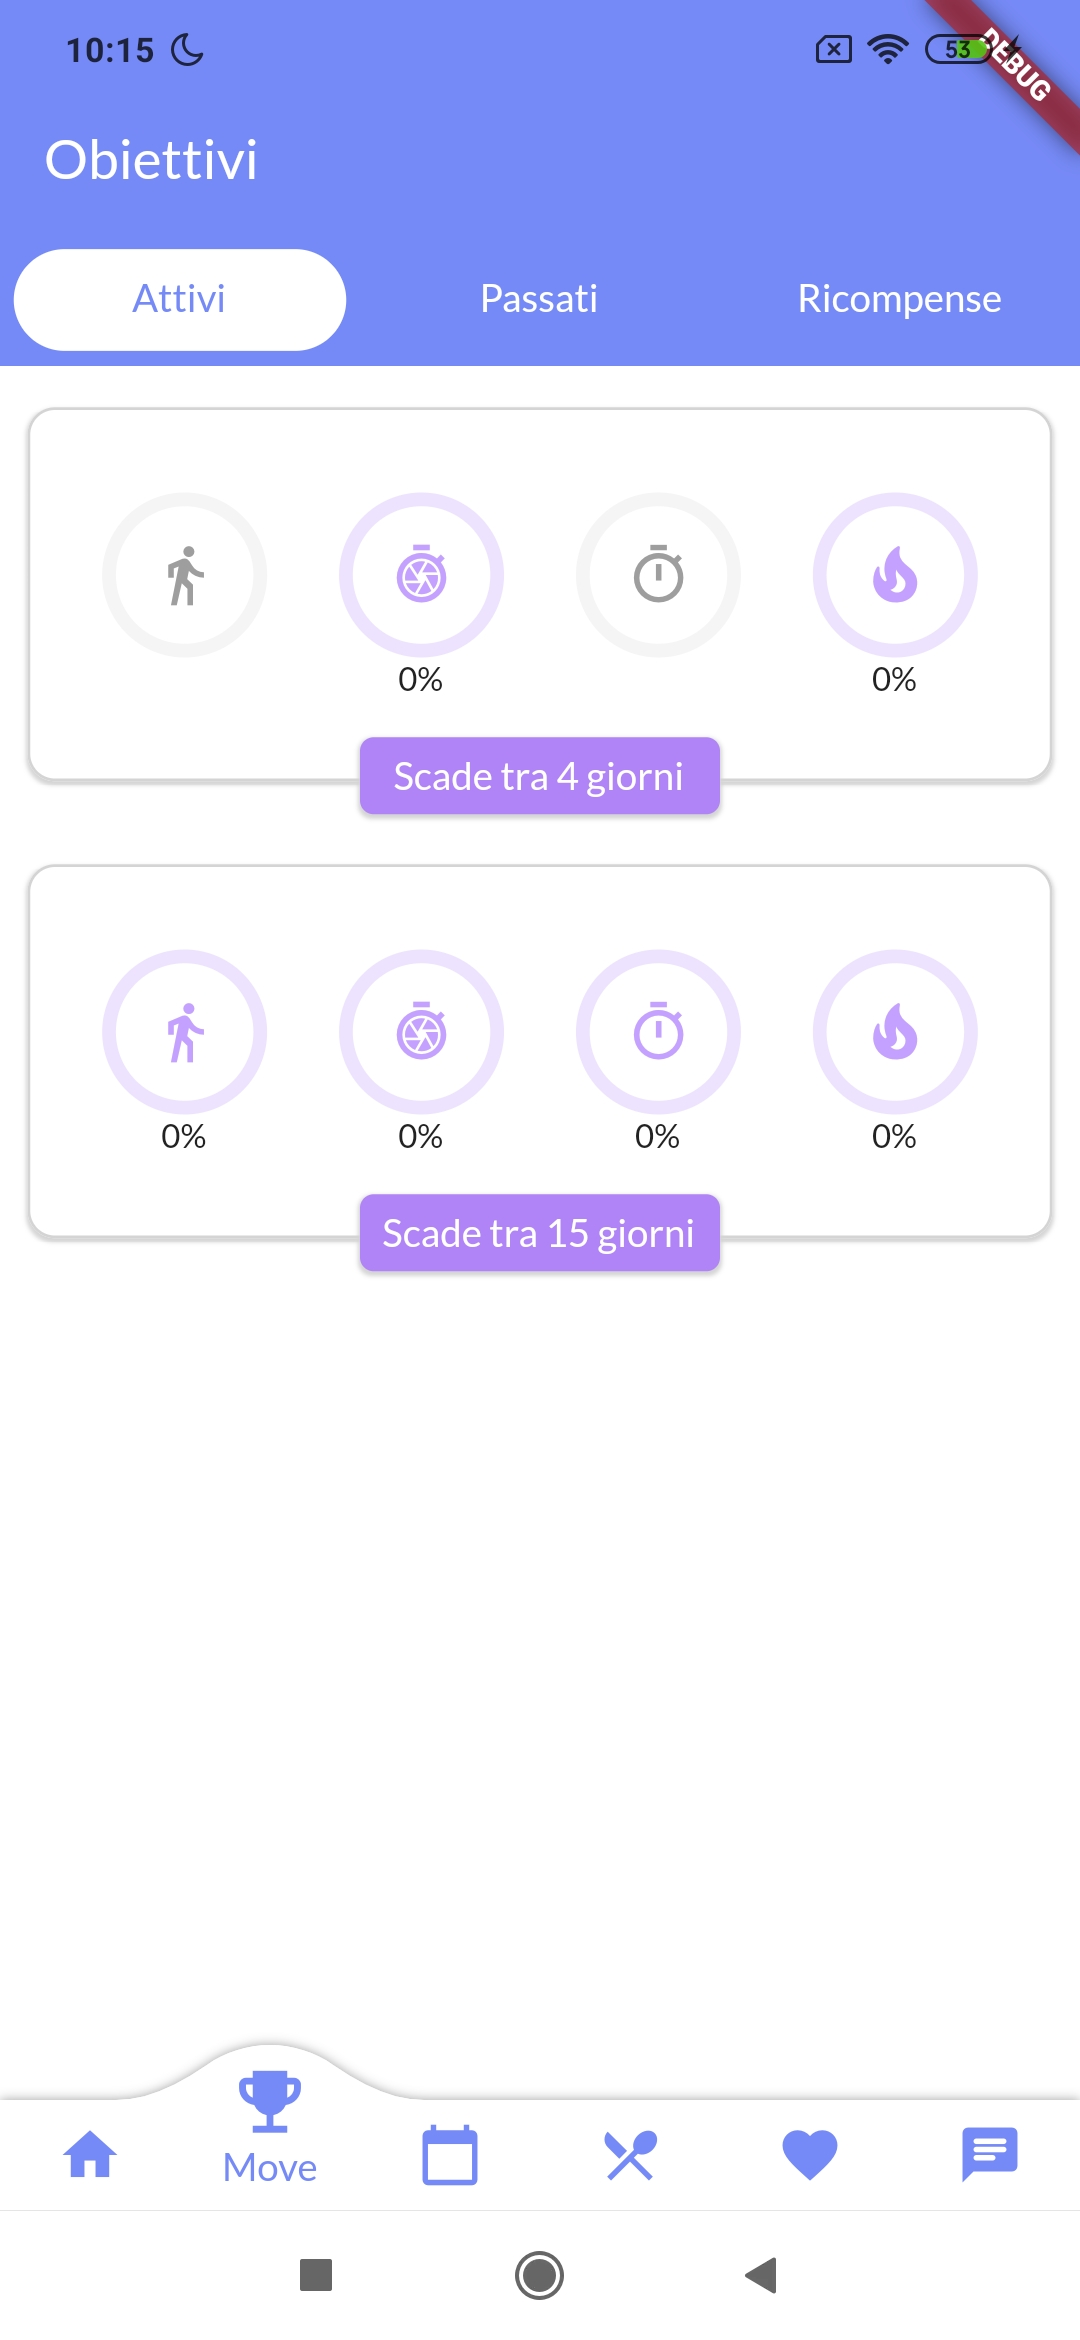
\includegraphics[width = 4cm]{app_screenshot/active_goals.jpg}} 
\hspace{0.1cm}
\subfloat[Obiettivi passati non raggiunti]{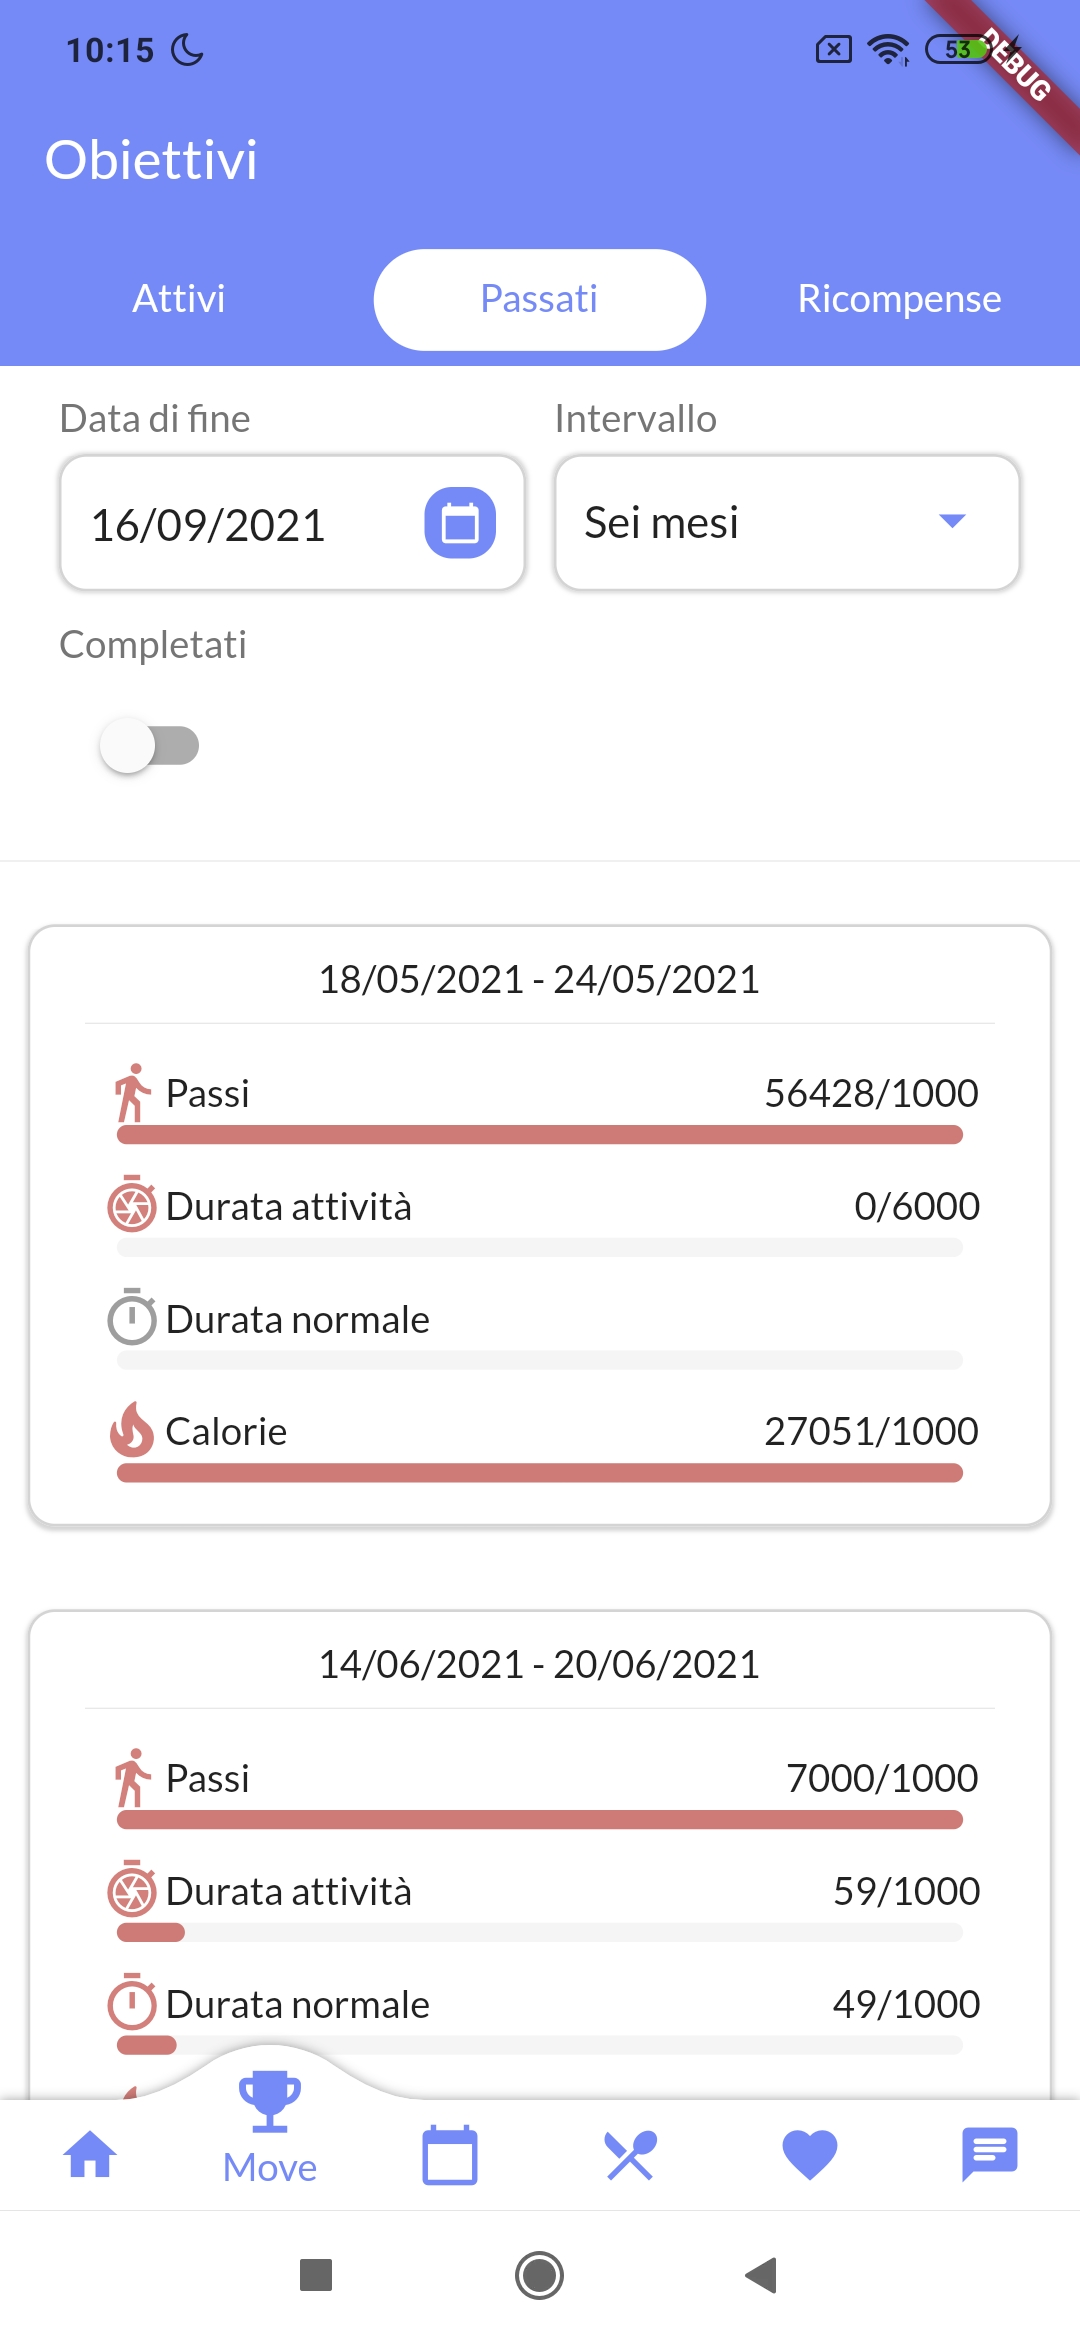
\includegraphics[width = 4cm]{app_screenshot/not_achieved_goals.jpg}}
\hspace{0.1cm}
\subfloat[Risultati]{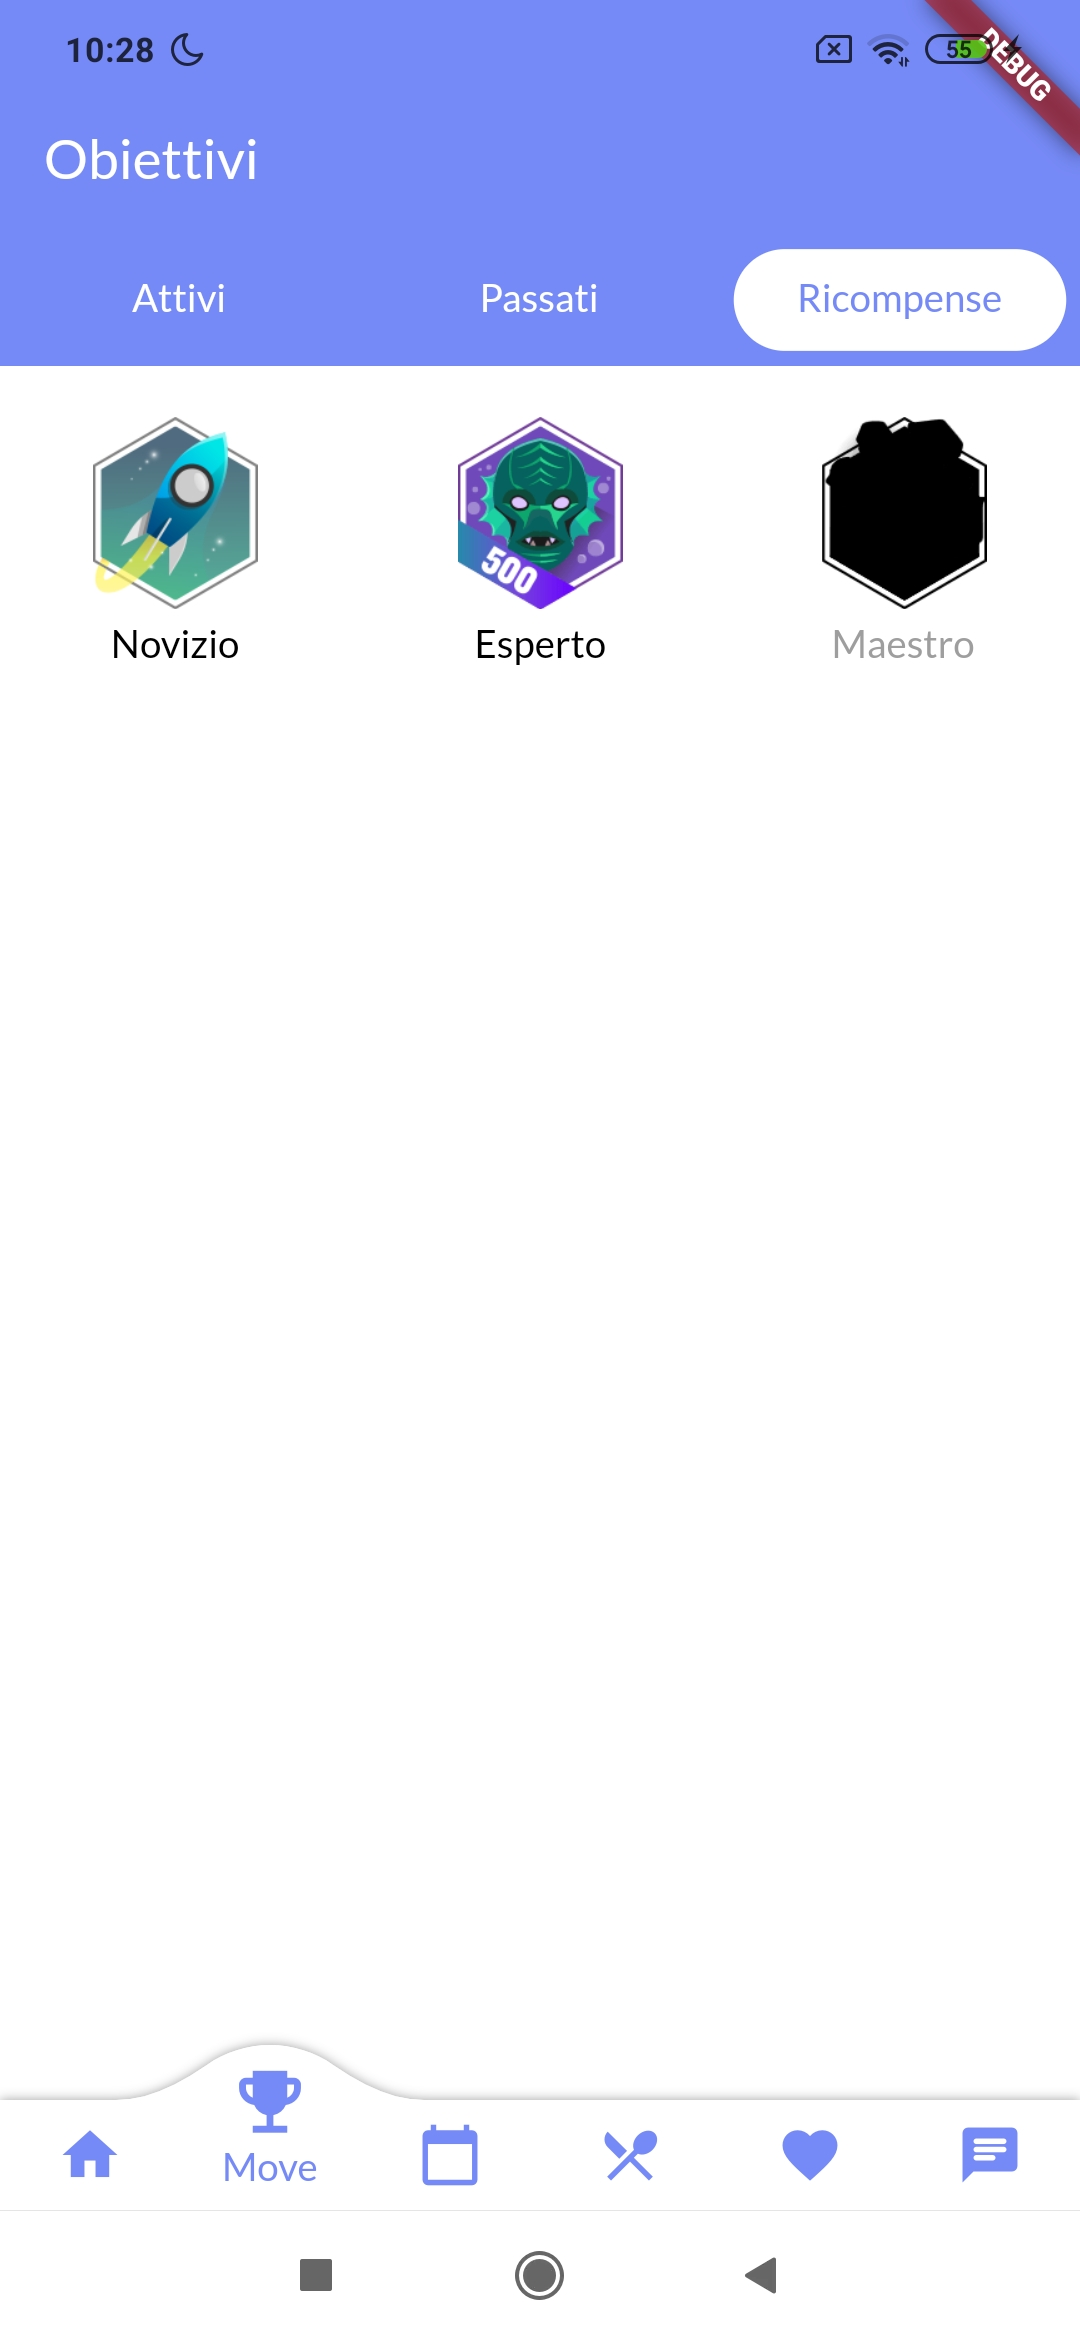
\includegraphics[width = 4cm]{app_screenshot/achievement.jpg}}
\caption{Schermata Move}
\end{figure}
\end{center}
%%%%%%%%%%%%%%%%%%%%%%%%%%%%%%%%%%%%%%%%%%%%%%%%%%%%%
\subsection{Agenda}
Questa schermata è raggiungibile dalla barra di navigazione. Tale schermata è leggermente diversa nelle due applicazioni: i clienti possono vedere nel calendario sia gli appuntamenti sia gli obiettivi, mentre i coach vedono solamente gli appuntamenti in quanto non possiedono obiettivi.\\
Cliccando su un giorno del calendario vengono mostrate all'utente le card con obiettivi e appuntamenti di quel giorno, le card sono le stesse mostrate nell'\textit{Homepage}, si è potuto quindi riutilizzare buona parte del codice.\\
L'agenda è stata sviluppata in modo da essere altamente scalabile, è possibile infatti visualizzare gli eventi di tutto il mese o di settimana in settimana, inoltre nel caso in cui in futuro saranno aggiunti altri tipi di eventi sarà facile aggiungerli tra quelli visualizzati nel calendario.\\
La scalabilità è stata raggiunta utilizzando come oggetti da visualizzare nel calendario una lista di \textit{Event} e facendo un cast a runtime al tipo corretto di oggetto per costruire la card corretta.
\begin{lstlisting}[language=dart, firstnumber=1,caption={Costruzione delle card con individuazione a runtime del tipo}]
List<Widget> buildCards(List<Event> selectedElements, BuildContext context) {
    List<Widget> children = [];
    children.addAll(buildGoalsCards(
        selectedElements
            .where((element) => element is Goals)
            .map((e) => e as Goals)
            .toList(),
        context));
    children.addAll(buildAppointmentCards(
        selectedElements
            .where((element) => element is Appointment)
            .map((e) => e as Appointment)
            .toList(),
        context));
    return children;
  }
\end{lstlisting}
%%%%%%%%%%%%%%%%%%%%%%%%%%%%%%%%%%%%%%%%%%%%%%%%%%%%%
\begin{center}
\begin{figure}[H]
\subfloat[Agenda client]{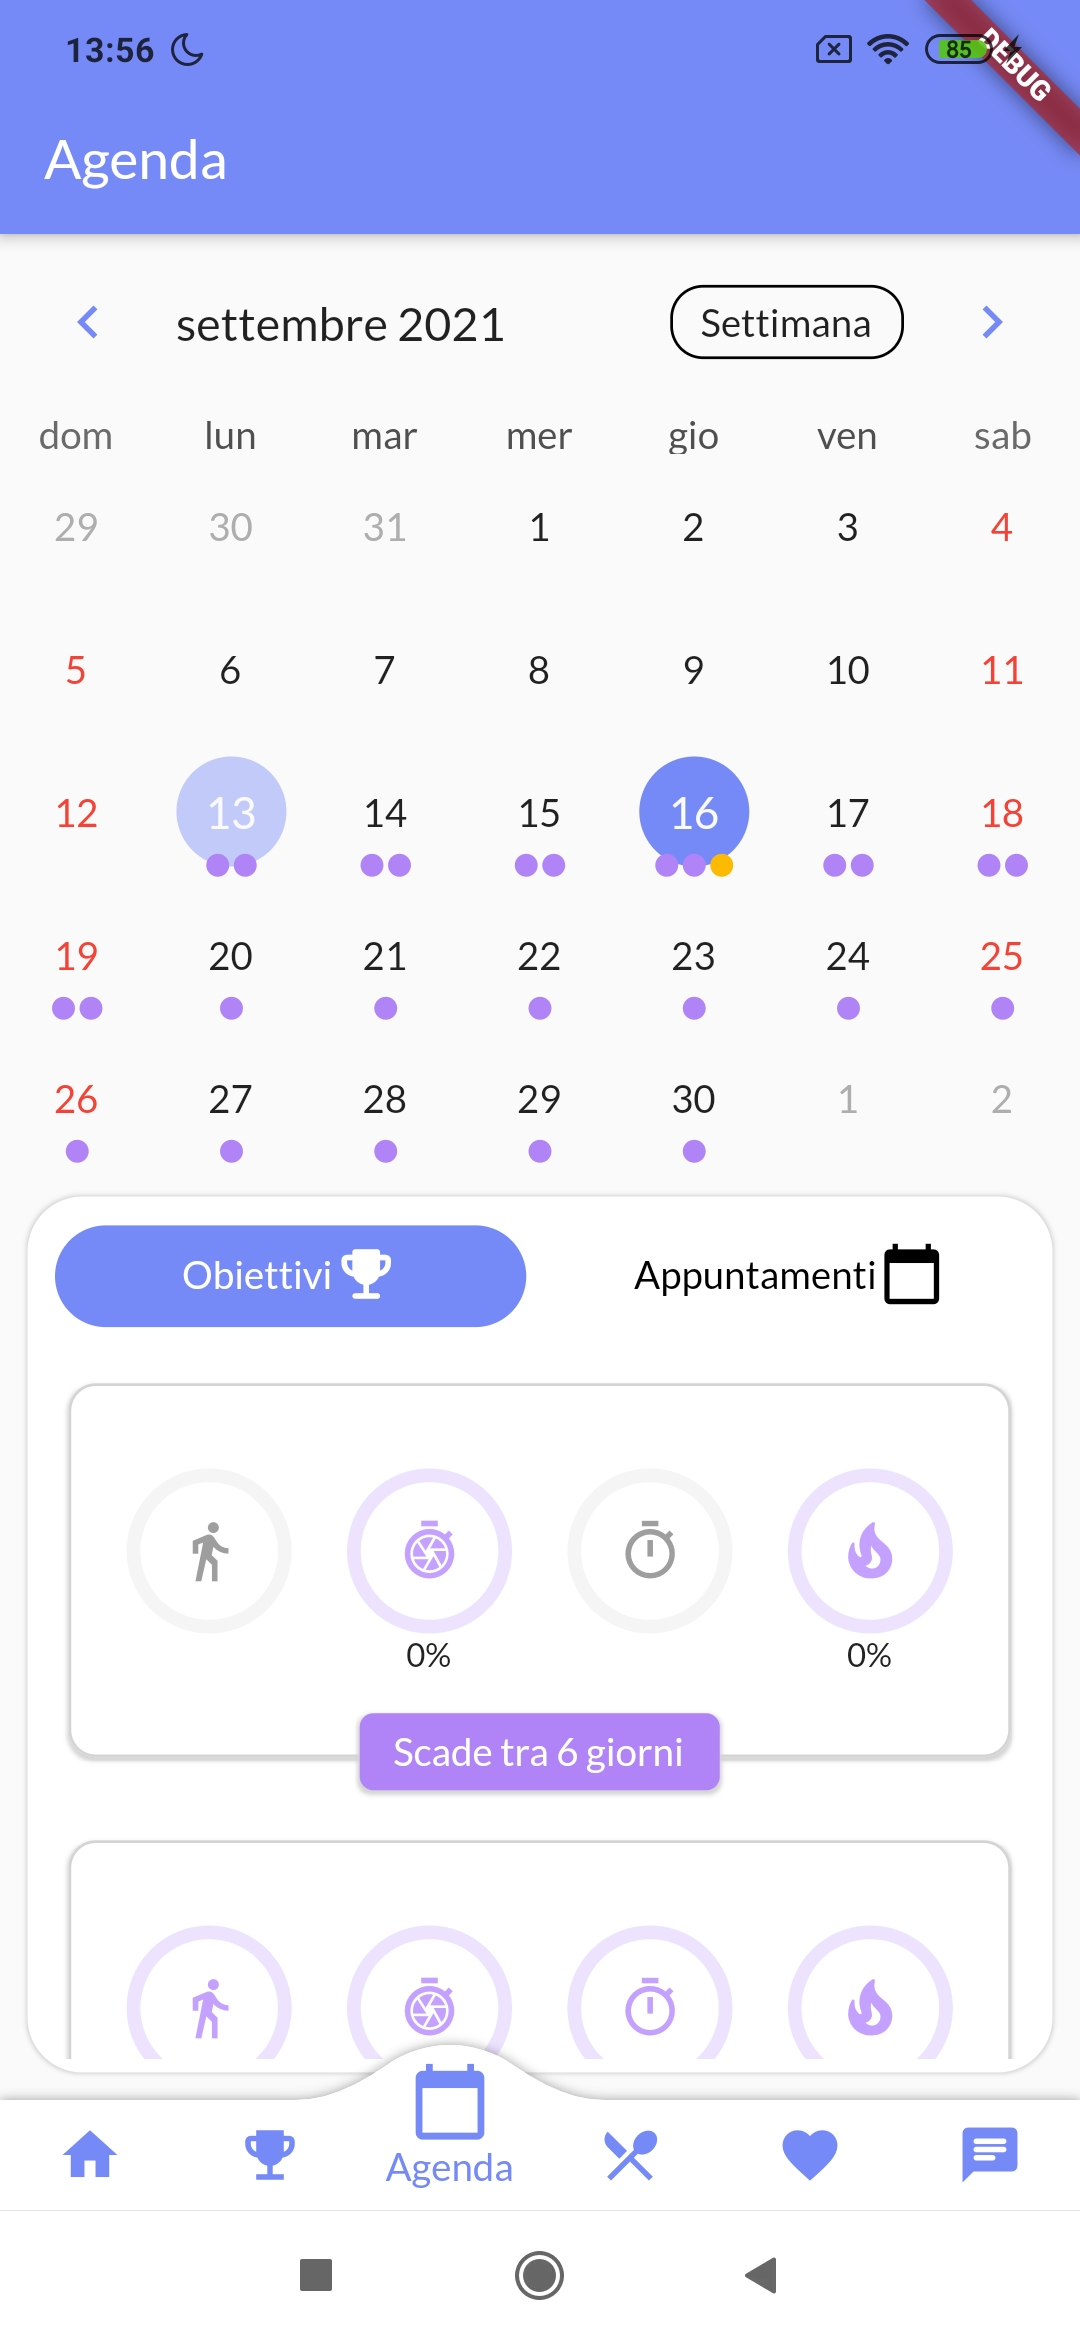
\includegraphics[width = 4cm]{immagini/app_screenshot/agendas_client.jpg}} 
\hspace{0.1cm}
\subfloat[Agenda client una settimana]{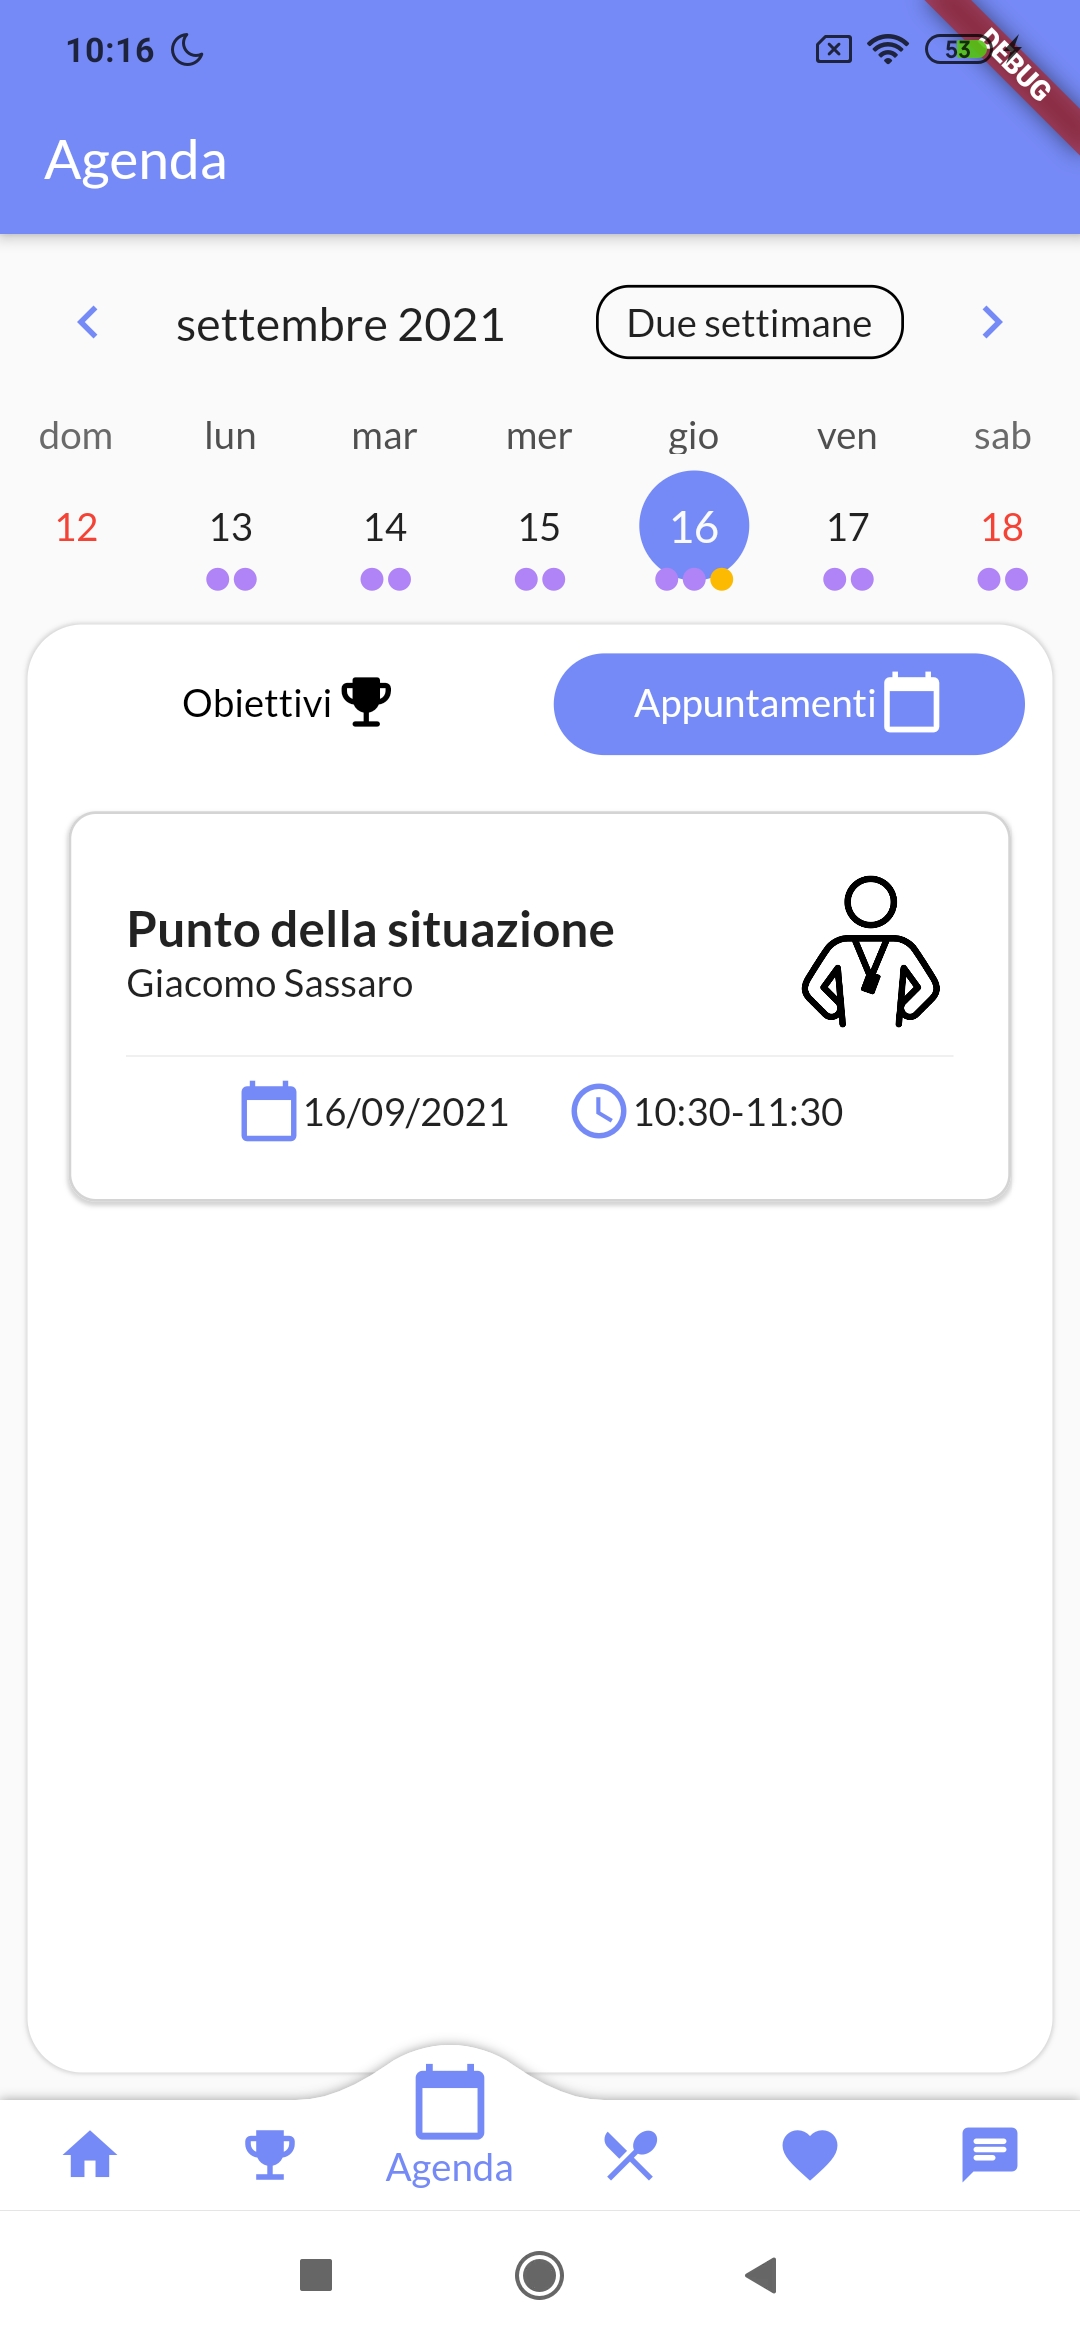
\includegraphics[width = 4cm]{immagini/app_screenshot/agenda_one_week.jpg}}
\hspace{0.1cm}
\subfloat[Agenda coach]{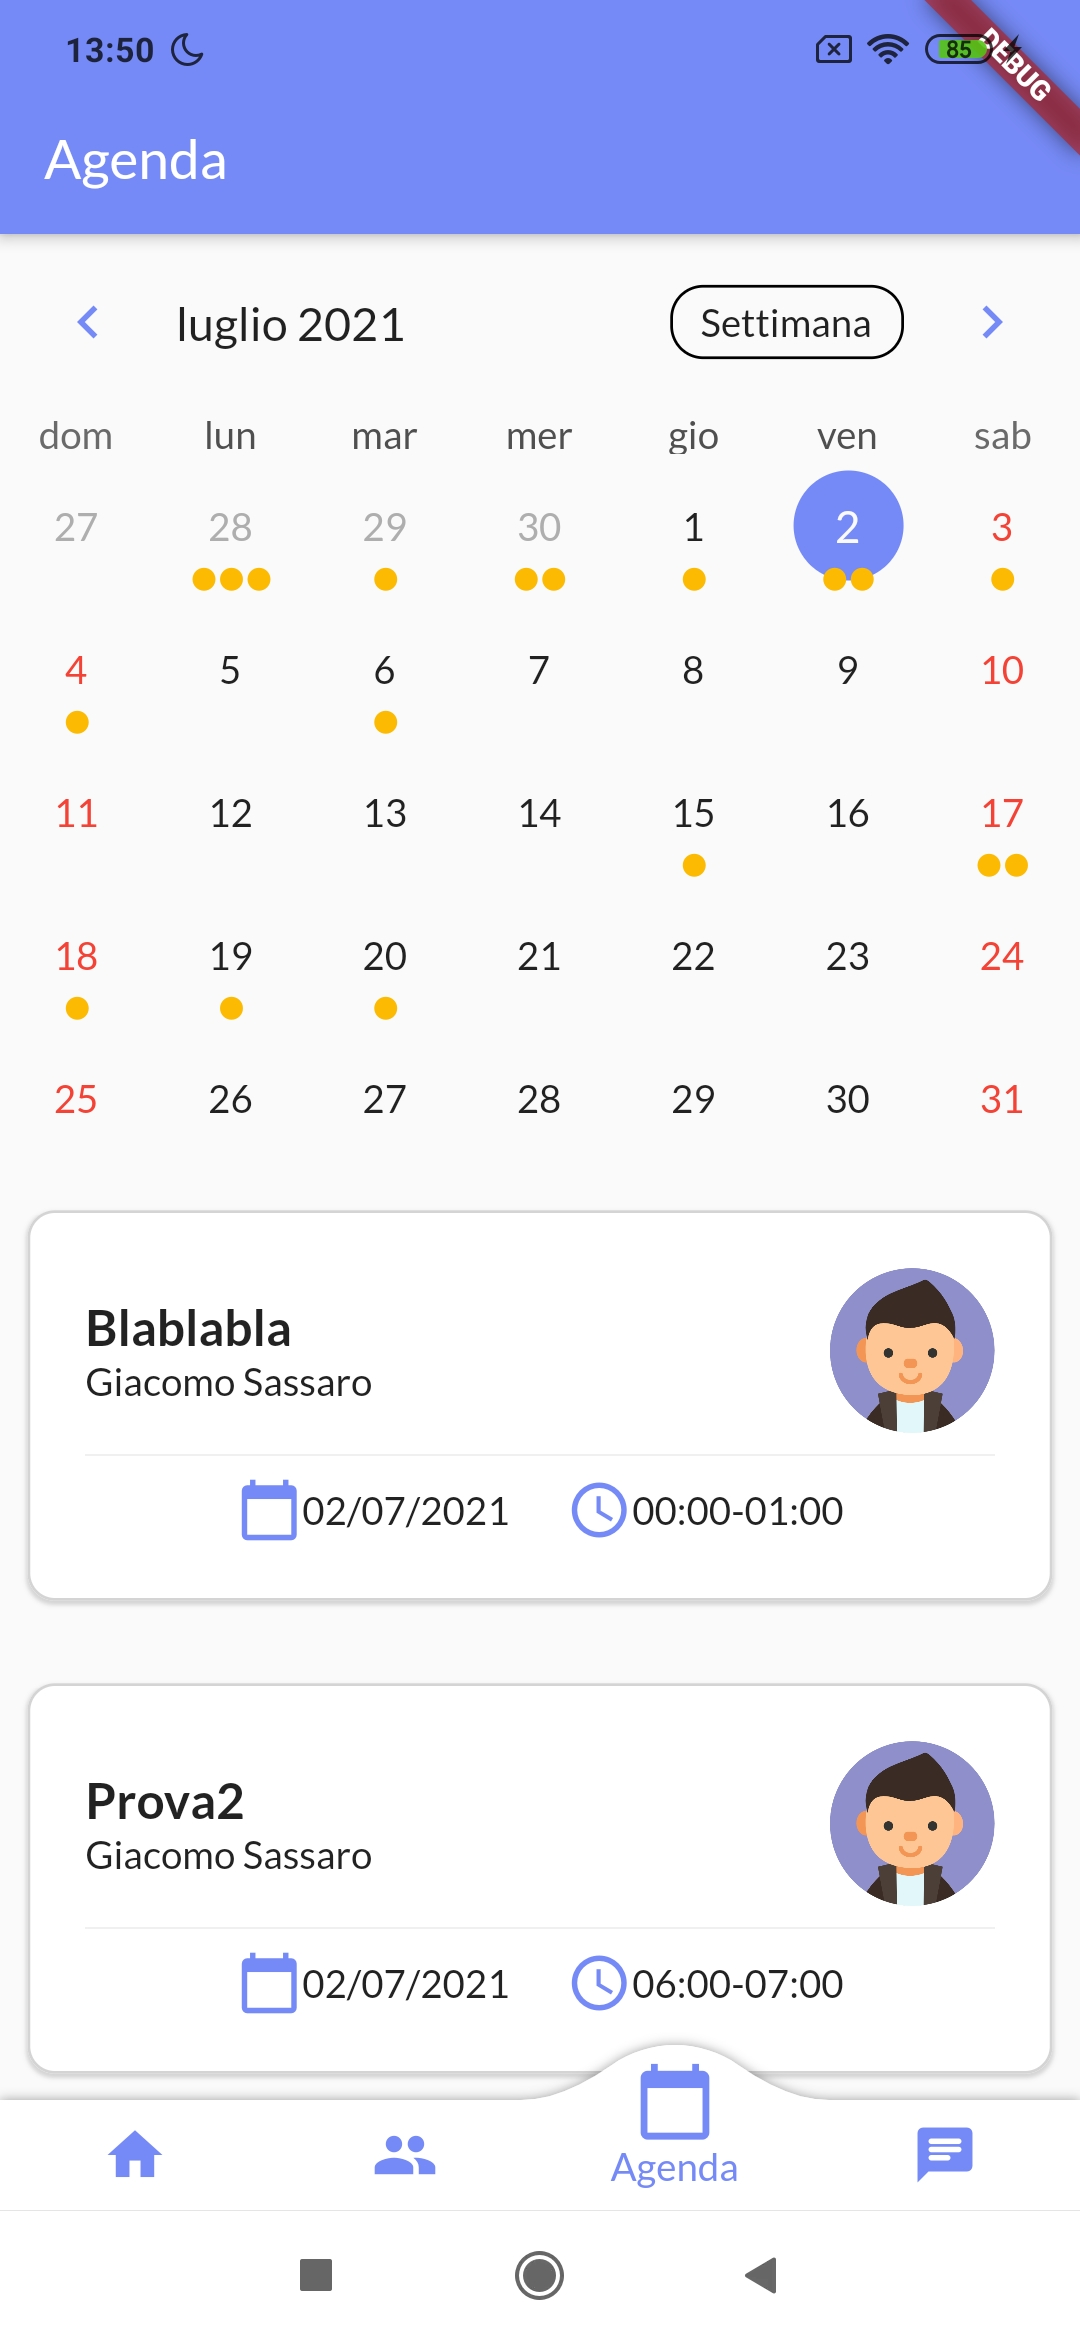
\includegraphics[width = 4cm]{immagini/app_screenshot/agendas_coach.jpg}}
\caption{Homepage e dettagli eventi}
\end{figure}
\end{center}
%%%%%%%%%%%%%%%%%%%%%%%%%%%%%%%%%%%%%%%%%%%%%%%%%%%%%
\subsection{Chat}
Quest'ultima schermata è raggiungibile in entrambe le applicazioni dalla barra di navigazione.\\
Per i clienti, arrivati in questa schermata, è subito visibile la chat con il proprio coach ed è possibile inviare messaggi o media. Nel caso invece dell'applicazione coach, arrivati nella schermata della chat, è visibile una lista con i contatti di tutti i clienti e solo cliccando sopra una di questa voce si aprirà la chat con il cliente.\\
Purtroppo, viste le poche ore rimaste a disposizione per lo sviluppo di tale sezione, al momento è solamente possibile inviare messaggi di testo, foto e video grazie ad una libreria già sviluppata per Flutter che sfrutta \textit{Google Firebase}. Inoltre non essendo ancora integrato Google Firebase con il nostro backend, gli utenti della chat sono simulati e non sono in alcun modo collegati agli account di LifestyleSync.\\
La libreria utilizzata per la costruzione della chat, nonostante inizialmente si fosse rivelata valida, manca di molte funzionalità. Infatti nella libreria è implementato solo il messaggio di tipo testuale e immagine, ho dovuto quindi fare un \gls{fork} per implementare il messaggio video e in futuro sarà sviluppato anche il messaggio vocale.
%*************************************************************************
\section{Applicazione coach}
L'applicazione coach è stata sviluppata quando lo sviluppo dell'applicazione client era già iniziato da alcune settimane, buona parte delle componenti e delle schermate è stato quindi possibile riutilizzarlo apportando poche modifiche al codice. Si è deciso infatti di mantenere la stessa \gls{codebase} per entrambe le applicazioni e sfruttare i flavors.\\
La principale differenza di quest'app da quella dei clienti è che qui non sono presenti le schermate \textit{Move}, \textit{Food} ed \textit{Health} in quanto un coach non possiede obiettivi propri.\\
Nell'app coach è però presente una schermata in cui il coach può vedere tutti i suoi clienti con i relativi obiettivi a loro assegnati.\\
%%%%%%%%%%%%%%%%%%%%%%%%%%%%%%%%%%%%%%%%%%%%%%%%%%%%%
\begin{center}
\begin{figure}[H]
\subfloat[Homepage coach]{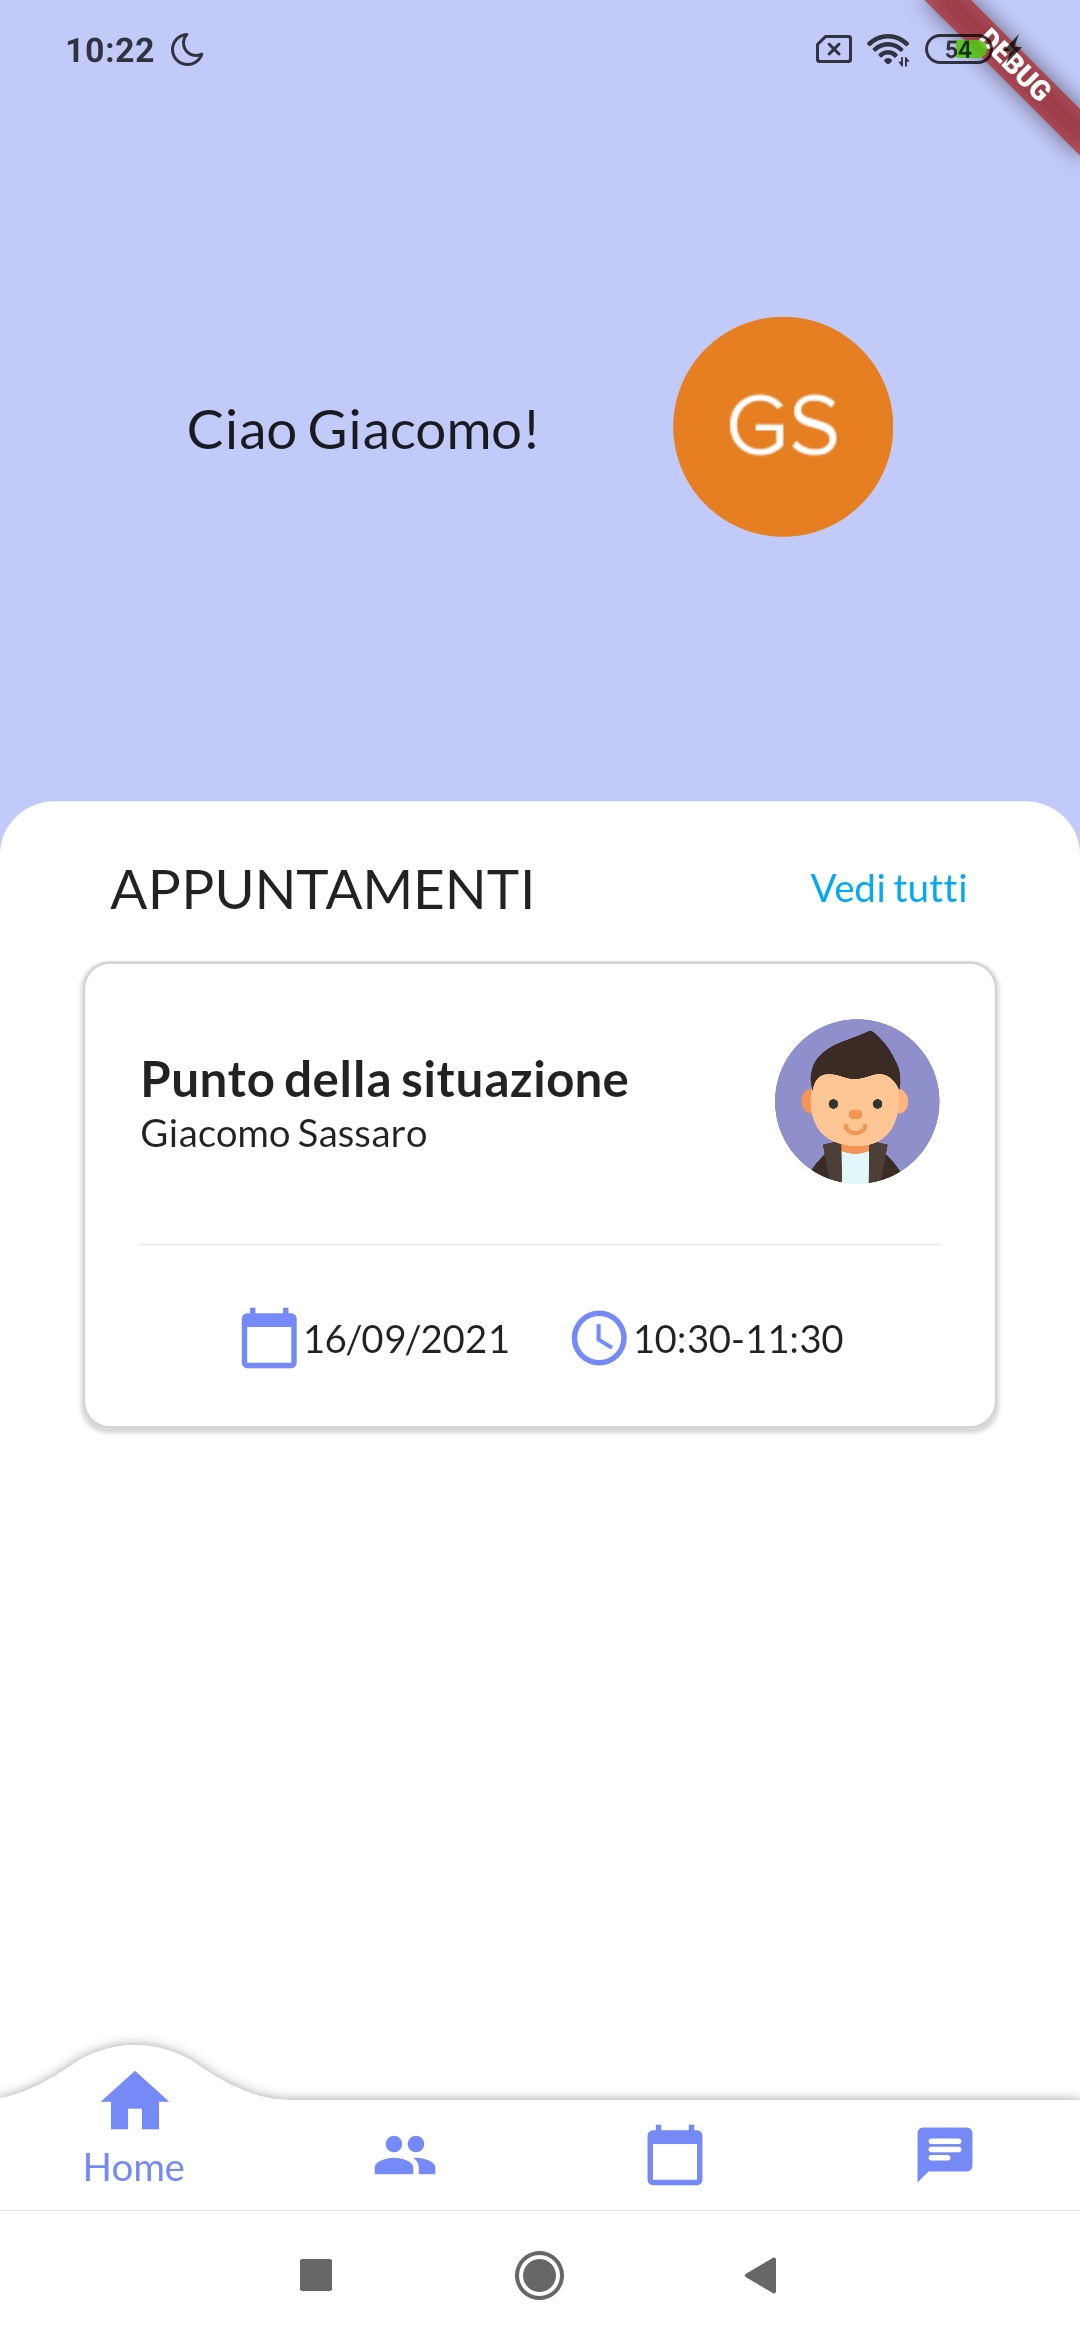
\includegraphics[width = 4cm]{immagini/app_screenshot/homepage_coach.jpg}} 
\hspace{0.1cm}
\subfloat[Lista clienti]{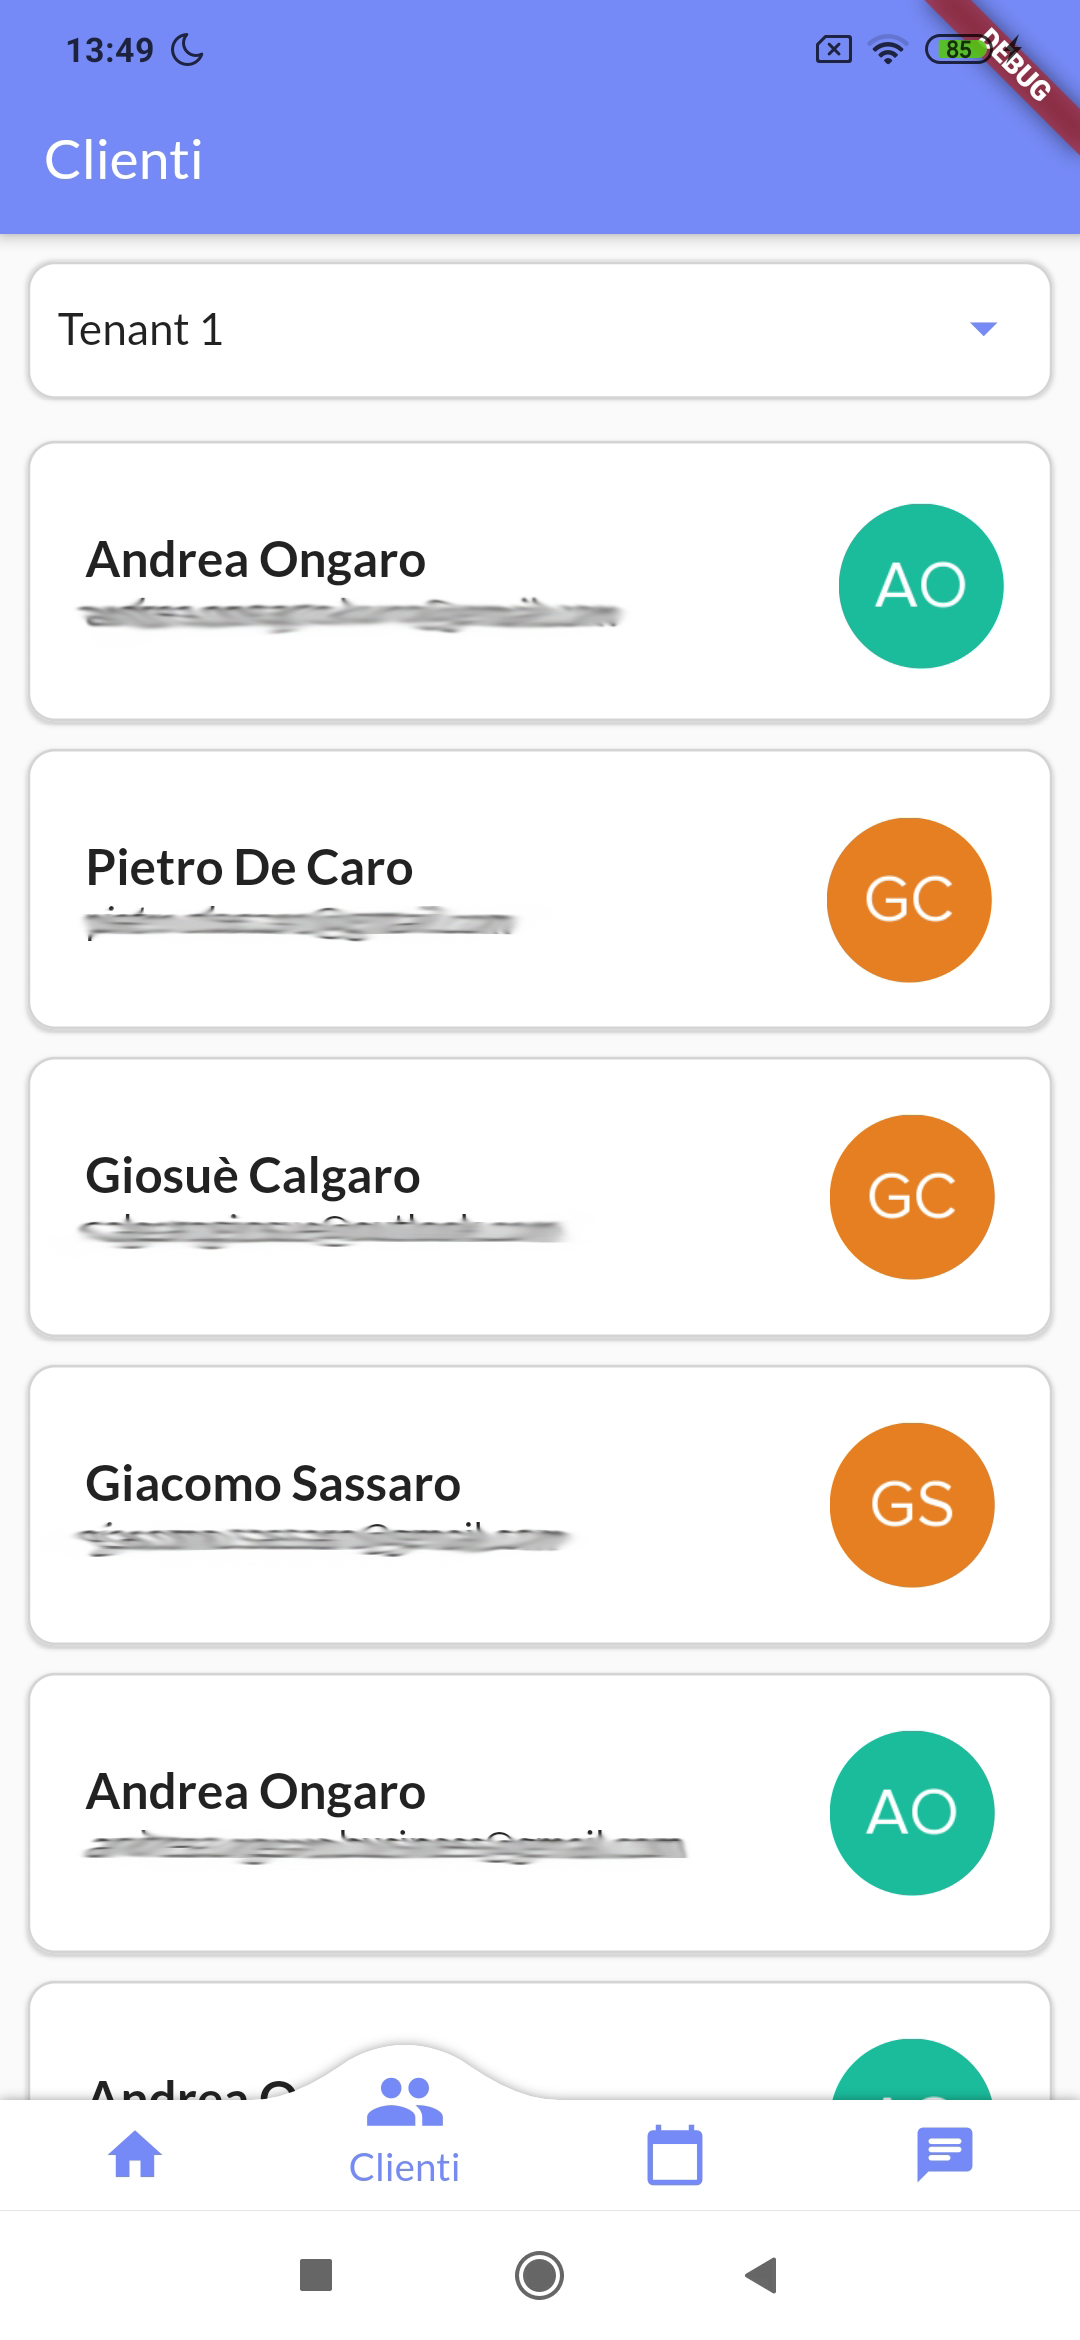
\includegraphics[width = 4cm]{immagini/app_screenshot/clients_coach.png}}
\hspace{0.1cm}
\subfloat[Dettaglio cliente]{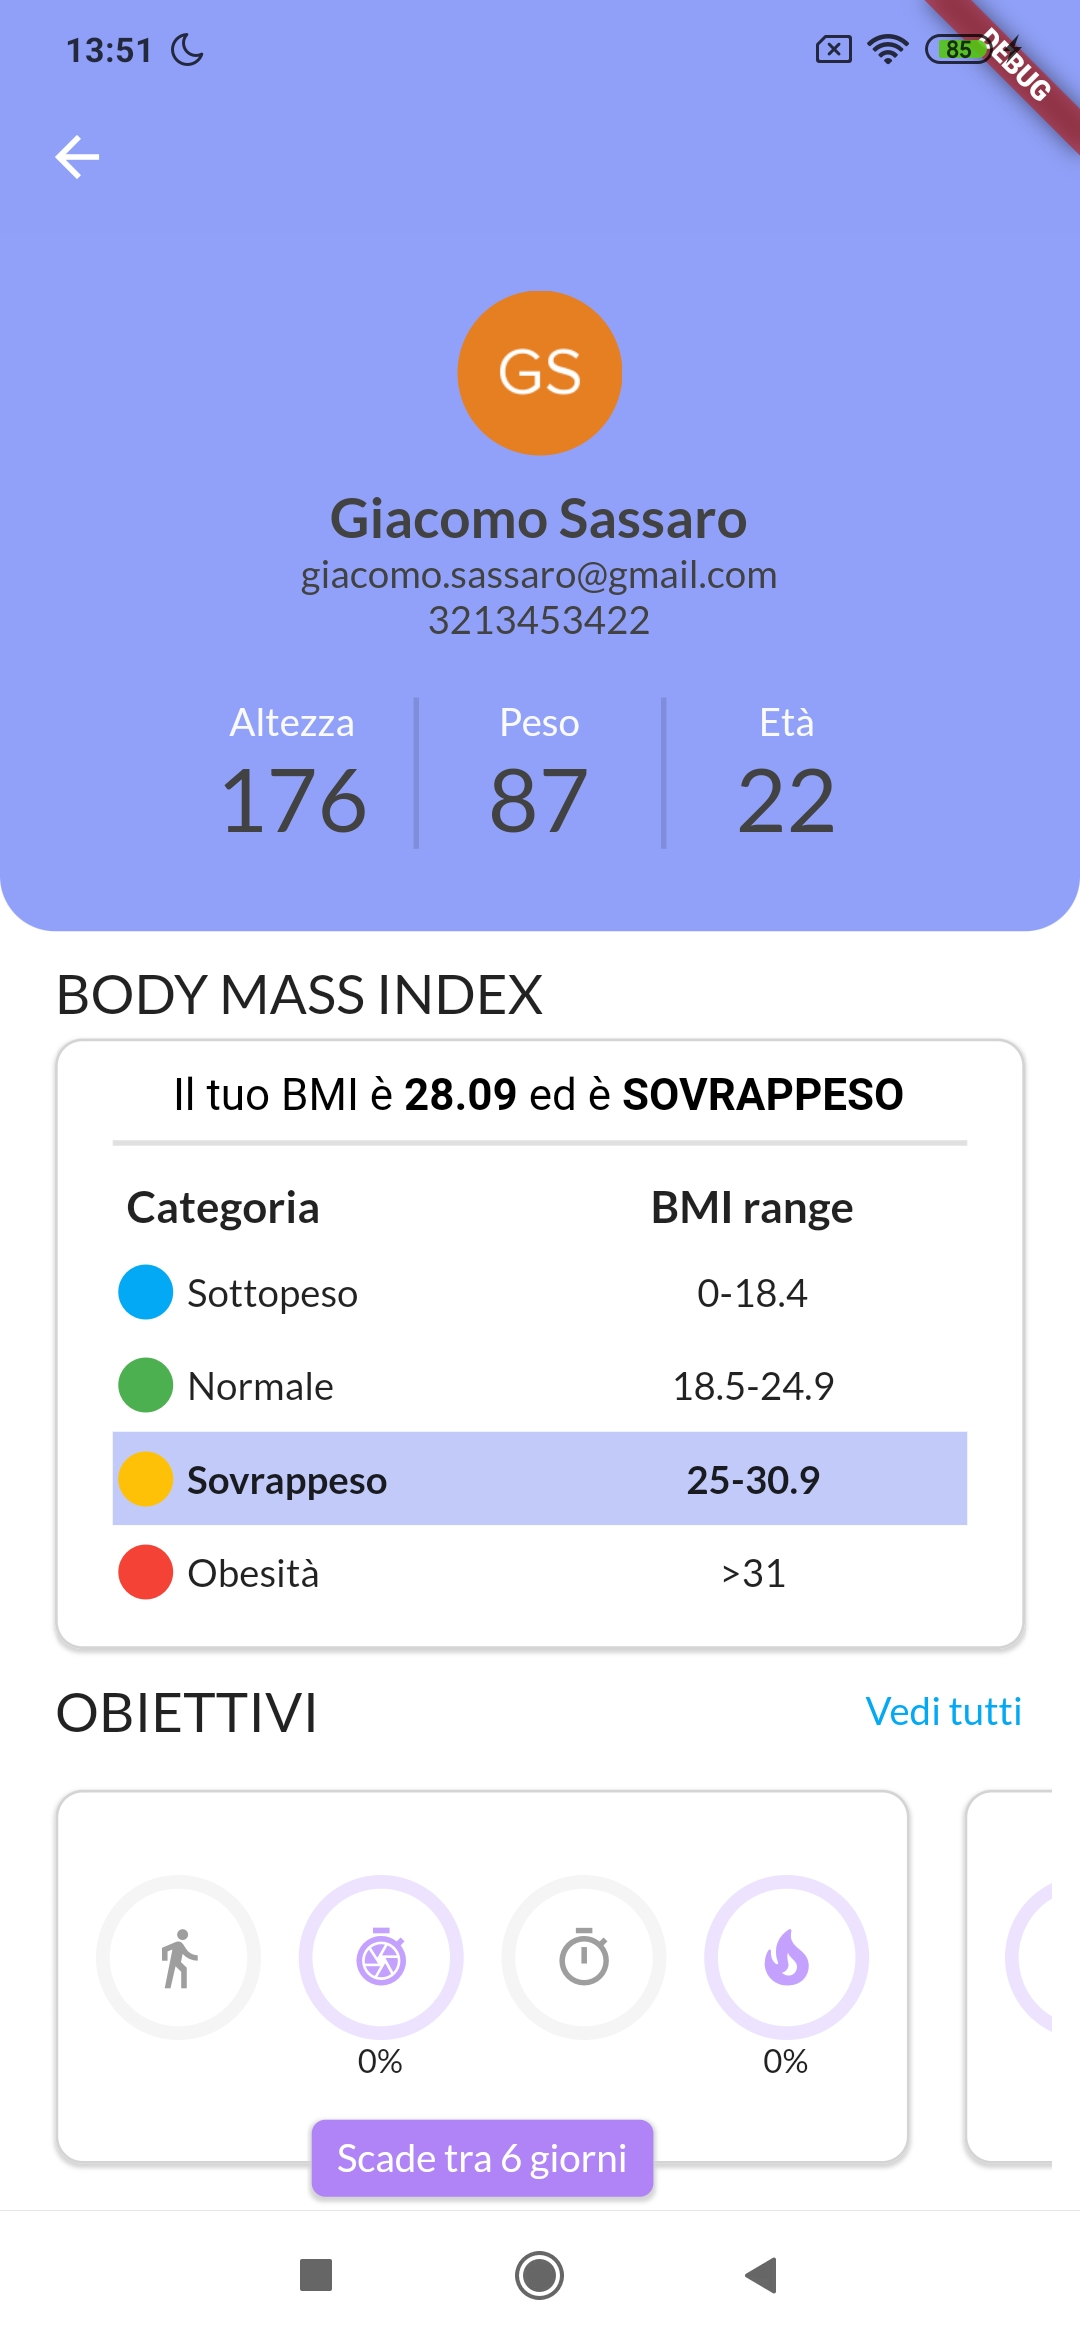
\includegraphics[width = 4cm]{immagini/app_screenshot/client_details_coach.jpg}}
\caption{Schermate app coach}
\end{figure}
\end{center}
%%%%%%%%%%%%%%%%%%%%%%%%%%%%%%%%%%%%%%%%%%%%%%%%%%%%%
